\documentclass[a4paper,12pt]{ctexbook}
\usepackage[utf8]{inputenc}
\usepackage{ctex}
\usepackage{graphicx}
\usepackage{amsfonts}
\usepackage{amsmath}
%\numberwithin{equation}{section}公式按章节编号
\usepackage{amsthm}
\usepackage{amssymb}
\usepackage[mathscr]{euscript}
\usepackage{geometry}
\usepackage{amssymb}
\usepackage{graphicx}
\usepackage{subfigure}
\geometry{a4paper,left=2.5cm,right=2.5cm,top=2.5cm,bottom=2.5cm}
\newtheorem{lemma}{\hspace{2em}引理}[section]%定义引理格式,用节标题编号
\newtheorem{theorem}[lemma]{\hspace{2em}定理}%定理和引理统一编号
\newtheorem{corollary}[lemma]{\hspace{2em}推论}
\newtheorem{proposition}[lemma]{\hspace{2em}命题}
\renewcommand{\proofname}{\indent\bf 证明}

\begin{document}
%	\author{Bruce E. Sagan}
%	\title{The Art of Counting(计数的艺术)}
%	\date{}
%	\maketitle
%	\newpage
\setcounter{chapter}{2}


\chapter{普通型生成函数计数}
	\begin{center}
		(杜玉洁 \quad 翻译)
	\end{center}



本章引入计数工具中最重要的技巧:生成函数. Wilf关于生成函数的性质写了一整本书. 现有数种不同类型的生成函数, 我们从最简单的普通型生成函数开始. 在第四、七、八章我们将处理其他类型的生成函数. 对于所有类型生成函数的研究, 基本的观点都是拿出一列我们感兴趣的数, 然后用代数对象, 也即多项式或形式幂级数来替代它. 这样做的好处是, 我们可以用代数对象所具有的性质来研究初始序列. 这使得序列的结果的证明有如下优点:

(1)证明会非常短.

(2)许多证明可以直接计算而不需要其他的方法.

(3)有时没有其他已知方法来获取给定的结果.

\section{生成多项式}
令$x$为变量. 复数序列\[
a_{0},a_{1},a_{2},\dots,a_{n} \tag{3.1}
\]有普通生成多项式
\[
f(x)=a_{0}+a_{1}x+a_{2}x^{2}+\cdots +a_{n}x^{n}=\sum_{k=0}^{n}a_{k}x^{k}.
\]在这里, “普通”是为了区别于其他类型的生成多项式. 因为我们只在这一章中处理普通生成多项式的情况, 我们经常去掉形容词. 注意$f(x)$是复数域上一元多项式环$\mathbb{C}[x]$中的元素, $x$的系数为复数. 我们也称$f(x)$为序列(3.1)的生成函数, 因为它是可数项序列(但是可能非有限项)生成函数的特殊情况. 这种更一般的设定将在3.3节中讨论.

我们从一个简单的例子开始讨论, 考虑帕斯卡三角形的一行中的二项式系数\[
\binom{n}{0},\binom{n}{1},\binom{n}{2},\cdots,\binom{n}{n}.
\]相应的生成函数为
\[f(x)=\sum_{k=0}^{n}\binom{n}{k}x^{k}.\]
特别地, 当$n=4$时, 我们有
\[f(x)=1+4x+6x^{2}+4x^{3}+x^{4}=(1+x)^{4}.\]
这就是众所周知的二项式定理. 我们给出这一结果的两种证明, 一种是组合方法, 另一种是代数运算.
\begin{theorem}[二项式定理]
	对于$n\in \mathbb{N}$, 有
	\[\sum_{k=0}^{n}\binom{n}{k}x^{k}=(1+x)^{n}.\]
\end{theorem}
\begin{proof}
	(组合证明)用乘法分配律展开乘积
	\[(1+x)^{n}=\overbrace{(1+x)(1+x) \cdots(1+x)}^{n}. \] 我们得到$x^{k}$项是通过选取$k$项$x$和$n-k$项1.但是从$n$个对象中选$k$个的方法数为$\binom{n}{k}$,这就是乘积中$x^{k}$项系数.
\end{proof}

\begin{proof}
	(代数证明)我们对$n$做归纳. 当$n=0$时等式显然成立. 因此假设$n\geq 1$.注意, 根据二项式系数的性质, 我们可以将生成函数写作\[
	\sum_{k=0}^{n}\binom{n}{k}x^{k}=\sum_{k=-\infty}^{\infty}\binom{n}{k}x_{k}.
	\]这样做的好处在于不用处理求和的界. 现在利用定理1.3.3(a)中关于二项式递归, 改变符号, 归纳得
\[
	\begin{aligned}
	\sum_{k}\binom{n}{k}x^{k} &=\sum_{k}\binom{n-1}{k-1}x^{k}+\sum_{k}\binom{n-1}{k}x^{k} \\
	&=x \sum_{k}\binom{n-1}{k-1} x^{k-1}+\sum_{k}\binom{n-1}{k}x^{k} \\
	&=x \sum_{k}\binom{n-1}{k}x^{k}+\sum_{k}\binom{n-1}{k}x^{k} \\
	&=x(1+x)^{n-1}+(1+x)^{n-1} \\
	&=(1+x)^{n}
	\end{aligned}
\]
\end{proof}
第一个证明展示了权重生成函数的乘法规则的使用, 我们将在3.4节讨论. 第二个证明表明有关生成函数的计算可以基于传统运算法则. 并且, 扩展求和域的技巧是我们经常使用以简便运算的方法之一. 我们现在想给出一个例子来展示一个生成函数是如何产生的, 到如何使用生成函数来给出其他结果的简单证明. 特别地, 在二项式定理中令$x=1$就得到
$$
\sum_{k=0}^{n}\binom{n}{k}=(1+1)^{n}=2^{n},
$$
这就是定理1.3.3的(c). 类似地, 我们令$x=-1$,就有
$$
\sum_{k=0}^{n}(-1)^{k}\binom{n}{k}=(1-1)^{n}=0^{n}=\delta_{0, n},
$$
这就是定理1.3.3的(d).

我们通过介绍第一类斯特林数的生成函数来结束本节. 这一结果的证明与二项式定理的代数证明类似, 留作习题. 第二类斯特林数的生成函数将在3.3节介绍形式幂级数之后讨论.
\begin{theorem}
	对于$n \in \mathbb{N}$ , 我们有\[
	\sum_{k=0}^{n} c(n, k) x^{k}=x(x+1)(x+2) \ldots(x+n-1).
	\]
\end{theorem}
在等式左边, 令$x=1$就得到特殊情况
$$
\# P([n])=\sum_{k} c(n, k)=n !.
$$
因此该命题可以看做是定理1.2.1的一般化. 这样的扩展被称为$q$-模拟, 将在下一节讨论.
\section{统计量与$q$-模拟}
一种构造生成函数的方法是通过使用统计量与$q$-模拟. 因为超几何级数理论与变量$q$的关系通常被用于这些生成函数. 这是一个助记符选择, 因为有时, 正如我们将在下面看到的, $q$代表素数$p$的幂. 目前还没有对q-模拟的正式定义, 因此我们将用一个例子开始, 将说明我们最终给出的元定义.

集合$S$上的{\kaishu 统计量}就是$S\rightarrow \mathbb{N}$的函数st. 因为统计量的值域为$\mathbb{N}$, 因此我们可以为有限集合$S$定义相应的生成多项式
$$
f(q)=\sum_{s \in S} q^{{\rm st} s} .
$$
这一生成函数有时被称为st在 $S$上的{\kaishu 分布 }, 因为它也可以被写作
$$
f(q)=\sum_{k \geq 0} a_{k} q^{k}
$$
其中$a_{k}$ 为$s \in S$中满足st $s=k$ 的元素个数, 这与概率论中随机变量的分布相似. 排列中最著名的统计量之一是逆序数.  排列$\pi=\pi_{1} \ldots \pi_{n} \in P([n])$ 有{\kaishu 逆序集}
$$
\text { Inv } \pi=\left\{(i, j) \mid i<j \text { and } \pi_{i}>\pi_{j}\right\} .
$$
我们可以认为该集合是指数对的集合, 其中$\pi$的相应元素并非它们的自然增长序. 注意, 我们使用指数对而非$\pi$的元素, 因为这可以更容易地将这个概念推广到允许重复的词. 比如说, 如果 $\pi=\pi_{1} \pi_{2} \pi_{3} \pi_{4} \pi_{5}=41532$, 那么
$$
\operatorname{Inv} \pi=\{(1,2),(1,4),(1,5),(3,4),(3,5),(4,5)\} .
$$
 $\pi$ 的{\kaishu 逆序数}就是
$$
\operatorname{inv} \pi=\# \operatorname{Inv} \pi .
$$
我们经常使用最开始函数的约定, 首字母大写代表集合, 小写代表集合的基数. 继续我们的例子,  inv $41532=6$. 显然 inv: $P([n]) \rightarrow \mathbb{N}$是一个统计量, 并且它有一个非常有趣的生成多项式.
\begin{theorem}
对于 $n \geq 0$, 我们有
 $$
\sum_{\pi \in P([n])} q^{\operatorname{inv} \pi}=(1)(1+q)\left(1+q+q^{2}\right) \cdots\left(1+q+q^{2}+\cdots+q^{n-1}\right).
$$
\end{theorem}

\begin{proof}
	我们对$n$作归纳, 并且省去琐碎的基本情况. 对每一个 $\pi \in P([n])$ , 可以通过 $\sigma \in P([n-1])$ 获得, 只需在$\sigma$的元素之间形成的$n$个空(包括$\sigma_{1}$的前面和$\sigma_{n-1}$的后面的空)中插入$n$即可. 令$\sigma^{i}$表示把$n$放在距离右边的第$i$个空, 其中$\sigma_{n-1}$后面的空记为0.于是显然有
	$$
	\operatorname{inv} \sigma^{i}=i+\operatorname{inv} \sigma.
	$$用该等式然后进行归纳得到
	$$
	\begin{aligned}
	\sum_{\pi \in P([n])} q^{\mathrm{inv} \pi} &=\sum_{\sigma \in P([n-1])} \sum_{i=0}^{n-1} q^{\mathrm{inv} \sigma^{1}} \\
	&=\sum_{\sigma \in P([n-1])} q^{\mathrm{inv} \sigma} \cdot \sum_{i=0}^{n-1} q^{i} \\
	&=(1+q)\left(1+q+q^{2}\right) \cdots\left(1+q+q^{2}+\cdots+q^{n-1}\right).
	\end{aligned}
	$$
\end{proof}
将$q=1$代入此结果得到$$
\# P([n])=\sum_{\pi \in P([n])} 1=n !
$$
这就是定理1.2.1的第二条内容.

现在我们已经遇到了一些q-模拟(尽管我们还没有这样命名), 它们的元定义会更有意义. 一个组合对象$\mathcal{O}$ 的{\kaishu q-模拟}就是 $\mathcal{O}(q)$满足
$$
\lim _{q \rightarrow 1} \mathcal{O}(q)=\mathcal{O}.
$$
注意 $\mathcal{O}$ 可以是许多东西:一个数, 一个定义或者一个定理. 比如 $n \in \mathbb{N}$ 的标准$q$-模拟是多项式
\begin{equation}
	[n]_{q}=1+q+q^{2}+\cdots+q^{n-1}\tag{3.2}
\end{equation}

显然$[n]_{1}=n .$$n$的另一可能的$q$-模拟是有理函数$\left(1-q^{n}\right) / (1-q) .$ 在这种情况下我们不能直接代入$q=1$, 而是必须要取极限. 当然, 商和 $[n]_{q}$ 在 $q \neq 1$时是相等的. 另一  $q$-模拟是 $q$-阶乘
$$
[n]_{q} !=[1]_{q}[2]_{q} \ldots[n]_{q} .
$$
因此定理3.2.1可被重新表述为
$$
\sum_{\pi \in P([n])} q^{i n v \pi}=[n]_{q} !.
$$
注意, 有时我们把$[n]_{q}$ 写作 $[n]$.这可能与$[n]$ 作为集合引起混淆, 因此我们只在清楚知道到底代表着什么时才使用此简便记号. 类似地, 在不致引起混淆时我们也可删除下标$q$.

还有另一著名的统计量, 用$[n]_{q} !$作为其分布.  $\pi \in P([n])$的{\kaishu 降序集}为
\[
\operatorname{Des} \pi=\left\{i \mid \pi_{i}>\pi_{i+1}\right\}.\tag{3.3}
\]
相应的{\kaishu 降序数}为 $\operatorname{des} \pi= \# {\rm Des}\pi$.并且如果$i \in$ Des $\pi$ 当且仅当$(i, i+1) \in \operatorname{Inv} \pi$.我们也可以定义{\kaishu 升序集}Asc $\pi$和{\kaishu 升序数}asc $\pi$, 只需调转(3.3)中不等号的方向. 继续我们之前的例子, 有  Des $41532=\{1,3,4\}$并且 des $41532=3$.  $\pi$ 的{\kaishu 主要指标}为
$$
\operatorname{maj} \pi=\sum_{i \in \text { Des } \pi} i .
$$
因此 maj $41532=1+3+4=8$.“主要指数”一词是由多米尼克·福阿塔[26]创造的, 以纪念英国军队的一名少校珀西·麦克马洪(Percy MacMahon), 他首先研究了这一统计数据[61].
\begin{theorem}
	对于$n\geq 0$, 我们有
	$$
	\sum_{\pi \in P([n])} q^{\operatorname{maj} \pi}=[n]_{q} !.
	$$
\end{theorem}
\begin{proof}
	我们像定理3.2.1一样证明, 但是现在 $\sigma$的空隙编号方式不同. 我们先给我们给$\sigma_{i}$和 $\sigma_{i+1}$(当$i$为降序)之间的空以及 $\sigma_{n-1}$之后的空编号, 从右到左从0开始编号. 然后给剩下的空编号, 从左到右用$\operatorname{des} \sigma+1$, des $\sigma+2, \ldots, n-1$进行编号. 例子见证明后.

	令 $\sigma^{(j)}$ 表示把$n$放在第$j$个位置后的结果. 我们称
\[
	\operatorname{maj} \sigma^{(j)}=j+\operatorname{maj} \sigma \tag{3.4}
\]
	事实上, 如果空$j$是下降位或者在$\sigma$的最后, 那么插入$n$只会移动$j$下降到右侧并包括给定下降一个位置的右侧. 通过定义主指标, maj $\sigma$总共增加了$j$. 如果空$j$是在上升位或者 $\sigma$的开始, 那么插入$n$增加了一个新的下降位, 并且把下降位移到空的后面某一位置的右边. 容易验证, 如果在空$j$插入$n$导致maj $\sigma$增加了$j$, 那么在空$j+1$插入$n$导致maj $\sigma$增加$j+1$.由归纳法知等式(3.4)对每个$j$都成立. 证毕.
\end{proof}

继续前面的例子 $\sigma=41532$且 maj $\sigma=8$, 空的编号顺序如下:
$$
{ }_{4} 4_{3} 1_{5} 5_{2} 3_{1} 2_{0} \text {. }
$$
在每一个空依次插入6得到
\begin{table}[h]
	\centering
	\begin{tabular}{c||c|c|c|c|c|c}
		$j$ & 0 & 1 & 2 & 3 & 4 & 5 \\
		\hline$\sigma^{(j)}$ & 415326 & 415362 & 415632 & 461532 & 641532 & 416532 \\
		\hline maj $\sigma^{(j)}$ & 8 & 9 & 10 & 11 & 12 & 13
	\end{tabular}
\end{table}

有很多排列统计量的分布为 $[n]_{q} !$ , 这些统计数据被 Foata 称为 Mahonian. 可以参考文章
Babson 和 Steingrímsson [3] 的 Mahonian 统计列表.

找到了涉及置换的 $q$-模拟后, 读者可能会怀疑它们也存在于组合中. 对于整数$0 \leq k \leq n$, 定义{\kaishu $q$-二项式系数}或{\kaishu 高斯系数}为
$$
\left[\begin{array}{l}
n \\
k
\end{array}\right]_{q}=\frac{[n]_{q} !}{[k]_{q} ![n-k]_{q} !}
$$
和往常一样, 如果$k<0$或$k>n$, 令这一函数为0.比如
\[
\begin{aligned}
\left[\begin{array}{l}
4 \\
2
\end{array}\right] &=\frac{[4] !}{[2] ![2] !} \\
&=\frac{[4][3]}{[2][1]} \\
&=\frac{\left(1+q+q^{2}+q^{3}\right)\left(1+q+q^{2}\right)}{(1+q)} \\
&=1+q+2 q^{2}+q^{3}+q^{4}
\end{aligned}\tag{3.5}
\]
只给出定义并不清楚这是一个$q$-多项式还是有理函数. 但是利用归纳法及我们下一个结果就很清楚了. 注意, 这一定理给出了普通二项式系数递归的两个$q$-模拟. 这说明了一个一般原则, 即$q$-模拟不一定是唯一的, 正如我们在$[n]_{q} !$ 的 inv 和 maj 解释中也看到的.
\begin{theorem}
	我们有$$
	\left[\begin{array}{l}
	0 \\
	k
	\end{array}\right]_{q}=\delta_{0, k}
	$$
并且对$n \geq 1$, 有
$$
\begin{aligned}
\left[\begin{array}{l}
n \\
k
\end{array}\right]_{q} &=q^{k}\left[\begin{array}{c}
n-1 \\
k
\end{array}\right]_{q}+\left[\begin{array}{c}
n-1 \\
k-1
\end{array}\right]_{q} \\
&=\left[\begin{array}{c}
n-1 \\
k
\end{array}\right]_{q}+q^{n-k}\left[\begin{array}{c}
n-1 \\
k-1
\end{array}\right]_{q}
\end{aligned}
$$
\end{theorem}
\begin{proof}
	初始条件是平凡的. 我们将证明$q$-二项式的第一个递归, 剩下的留作练习. 使用 $q$-阶乘的定义并找到一个公分母得到
	$$
	\begin{aligned}
	q^{k}\left[\begin{array}{c}
	n-1 \\
	k
	\end{array}\right]+\left[\begin{array}{c}
	n-1 \\
	k-1
	\end{array}\right] &=\frac{[n-1] !}{[k] ![n-k] !}\left(q^{k}[n-k]+[k]\right) \\
	&=\frac{[n-1] !}{[k] ![n-k] !} \cdot[n] \\
	&=\left[\begin{array}{c}
	n \\
	k
	\end{array}\right].
	\end{aligned}
	$$
	证毕.
\end{proof}

下面我们给出二项式定理(定理3.1.1)的$q$-模拟. 令$q,t$为两个变量.
\begin{theorem}
	对于 $n \geq 0$我们有
	\[
	(1+t)(1+q t)\left(1+q^{2} t\right) \cdots\left(1+q^{n-1} t\right)=\sum_{k=0}^{n}q^{\binom{k}{2}} \left[\begin{array}{l}
	n \\
	k
	\end{array}\right]_{q} t^{k} .\tag{3.6}
	\]
\end{theorem}
\begin{proof}
	我们对$n$作归纳, $n=0$的情况很容易验证. 对于 $n>0$ 的情形, 我们用前面结果的第二个递推关系以及归纳假设有
	$$
	\begin{aligned}
	\sum_{k} q^{\binom{k}{2}} &\left[\begin{array}{l}
	n \\
	k
	\end{array}\right]_{q} t^{k}=\sum_{k} q^{\binom{k}{2}}\left[\begin{array}{c}
	n-1 \\
	k
	\end{array}\right]_{q} t^{k}+\sum_{k} q^{\binom{k}{2}+n-k}\left[\begin{array}{c}
	n-1 \\
	k-1
	\end{array}\right]_{q} t^{k} \\
	&=(1+t)(1+q t) \cdots\left(1+q^{n-2} t\right)+q^{n-1} t \sum_{k} q^{\binom{k-1}{2}}\left[\begin{array}{c}
	n-1 \\
	k-1
	\end{array}\right]_{q} t^{k-1} \\
	&=(1+t)(1+q t) \cdots\left(1+q^{n-2} t\right)+q^{n-1} t(1+t)(1+q t) \cdots\left(1+q^{n-2} t\right) \\
	&=(1+t)(1+q t) \cdots\left(1+q^{n-1} t\right),
	\end{aligned}
	$$这就是我们想要的结果.
\end{proof}

 $q$-二项式系数有许多种组合解释, 我们在这里展示其中两种. 假设$\lambda=\left(\lambda_{1}, \ldots, \lambda_{k}\right)$ 何 $\mu=$ $\left(\mu_{1}, \ldots, \mu_{l}\right)$是整数分拆, 如果$k \geq l$且当$i \leq l$时有 $\lambda_{i} \geq \mu_{i}$. 则称$\lambda$包含$\mu$, 记作 $\lambda \supseteq \mu$.换句话说, $\lambda$的杨图包含 $\mu$ 的杨图, 如果适当放置使它们的西北角对齐. 比如说,  $(5,5,2,1) \supseteq$ $(3,2,2)$ , 见图3.1, 阴影部分是 $\mu$的杨图, 包含在$\lambda$的杨图中. 符号 $\mu \subseteq \lambda$应该是不言自明的. 给定 $\mu \subseteq \lambda$, 也有相应的{\kaishu 倾斜分拆}
\[
\lambda / \mu=\{(i, j) \in \lambda \mid(i, j) \notin \mu\} .\tag{3.7}
\]
图 3.1 中 倾斜分拆的单元格是白色的.
\begin{figure}[h]
	\centering
	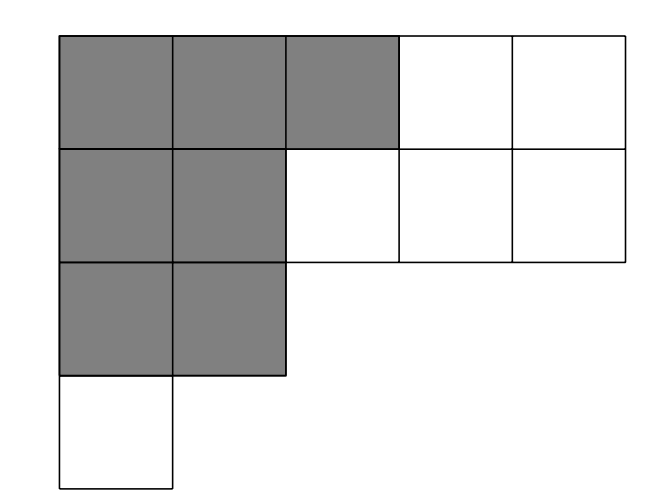
\includegraphics[width=0.5\linewidth]{./fig3/3-1.png}
	\caption{\label{chapter} $(5,5,2,1) \supseteq$ $(3,2,2)$的杨图}
\end{figure}

 $k \times l$矩形是整数分拆, 其重数表示法为$\left(k^{l}\right) $. 考虑包含在这一矩形的分拆集合
$$
\mathcal{R}(k, l)=\left\{\lambda \mid \lambda \subseteq\left(k^{l}\right)\right\}
$$
 $|\lambda|$是分拆 $\lambda$的部分数, 我们考虑生成函数$\sum_{\lambda \in \mathcal{R}(k, l)} q^{|\lambda|} $. 比如, 如果  $k=l=2$, 那么我们有

$$
\begin{array}{c||c|c|c|c|c|c}
\lambda \subseteq\left(2^{2}\right) & \emptyset & (1) & (2) & \left(1^{2}\right) & (2,1) & \left(2^{2}\right) \\
\hline q^{|\lambda|} & 1 & q & q^{2} & q^{2} & q^{3} & q^{4}
\end{array},
$$
因而
$$
\sum_{\lambda \in R(2,2)} q^{|\lambda|}=1+q+2 q^{2}+q^{3}+q^{4}.
$$
读者会注意到这一结果与(3.5)类似, 这并非巧合.
\begin{theorem}
	对于$k, l \geq 0$, 我们有
	$$
	\sum_{\lambda \in \mathcal{R}(k, l)} q^{|\lambda|}=\left[\begin{array}{c}
	k+l \\
	k
	\end{array}\right]_{q} .
	$$
\end{theorem}
\begin{proof}
	对$k$作归纳,  $k=0$的情况留给读者. 如果$k>0$且$\lambda \subseteq\left(k^{l}\right)$, 则有两种可能. 一种情况是$\lambda_{1}<k$并且$\lambda \subseteq\left((k-1)^{l}\right)$. 另一种情况是 $\lambda_{1}=k$, 此时 $\lambda$可以写作$\lambda=\left(k, \lambda^{\prime}\right)$ , 其中$ \lambda^{\prime}$ 是$\lambda$的不包含$\lambda_{1}$的分拆. 因此 $\lambda^{\prime} \subseteq\left(k^{l-1}\right)$. 注意在这种情况下$|\lambda|=\left|\lambda^{\prime}\right|+k$. 我们用归纳法及定理3.2.3得到
	\[
	\begin{aligned}
	\sum_{\lambda \in \mathcal{k}(k, l)} q^{|\lambda|} &=\sum_{\lambda \in \mathcal{R}(k-1, l)} q^{|\lambda|}+\sum_{\lambda^{\prime} \in \mathcal{R}(k, l-1)} q^{\left|\lambda^{\prime}\right|+k} \\
	&=\left[\begin{array}{c}
	k+l-1 \\
	k-1
	\end{array}\right]+q^{k}\left[\begin{array}{c}
	k+l-1 \\
	k
	\end{array}\right] \\
	&=\left[\begin{array}{c}
	k+l \\
	k
	\end{array}\right],
	\end{aligned}
	\]证毕.
\end{proof}

 对于第二种高斯多项式的组合解释, 需要一些线性代数的工具. 令$q$为素幂, 令 $\mathbb{F}_{q}$ 为具有$q$个元素 的伽罗瓦域. 令 $V$为 $\mathbb{F}_{q} $上维数$\operatorname{dim} V=n$的向量空间.
 元素. 我们用 $W \leq V$ 表示 $W$ 是 $V$的子空间. 令
$$
\left[\begin{array}{l}
V \\
k
\end{array}\right]=\{W \leq V \mid \operatorname{dim} W=k\}.
$$
维数为$k$的子空间与$k \times n$的满秩的 行最简形矩阵成一一对应. 比如说, 如果$n=4$ , $k=2$, 那么可能的矩阵为
$$
\begin{aligned}
&{\left[\begin{array}{llll}
	0 & 0 & 1 & 0 \\
	0 & 0 & 0 & 1
	\end{array}\right],\left[\begin{array}{llll}
	0 & 1 & * & 0 \\
	0 & 0 & 0 & 1
	\end{array}\right],\left[\begin{array}{llll}
	0 & 1 & 0 & * \\
	0 & 0 & 1 & *
	\end{array}\right]}, \\
~\\
&{\left[\begin{array}{llll}
	1 & * & * & 0 \\
	0 & 0 & 0 & 1
	\end{array}\right],\left[\begin{array}{llll}
	1 & * & 0 & * \\
	0 & 0 & 1 & *
	\end{array}\right],\left[\begin{array}{llll}
	1 & 0 & * & * \\
	0 & 1 & * & *
	\end{array}\right],}
\end{aligned}
$$
其中*表示$\mathbb{F}_{q}$的任意元素. 所以相应星图之一的子空间的数量是 $q^{s}$, 其中$s$ 是星星的数量. 因此
$$
\#\left[\begin{array}{c}
\mathbb{F}_{q}^{4} \\
2
\end{array}\right]=1+q+2 q^{2}+q^{3}+q^{4},
$$
在这一点上看来非常相似. 但是请注意, 与之前的情况相反, 这实际上代表一个整数而不是多项式, 因为 $q$是素幂. 当然, 这个例子是概括性的. 因为这个结果, 人们有时半开玩笑地称伽罗瓦域上只有一个元素的集合成为向量空间是不存在的.
\begin{theorem}
	如果$V$是$\mathbb{F}_{q}$维数为$n$的向量空间, 那么
	$$
	\#\left[\begin{array}{l}
	V \\
	k
	\end{array}\right]=\left[\begin{array}{l}
	n \\
	k
	\end{array}\right]_{q}.
	$$
\end{theorem}
 \begin{proof}
 	给定 $W \leq V$使得$\operatorname{dim} W=k$, 我们首先确定$W$的可能有序基$\left(\mathbf{v}_{1}, \mathbf{v}_{2}, \ldots, \mathbf{v}_{k}\right)$ 的数目. 注意, 因为 $\operatorname{dim} V=n$ , 我们有$\# V=\# \mathbb{F}_{q}^{n}=q^{n} $ .我们可以为 $\mathbf{v}_{1}$选出任意非零向量, 因此可以选择的数目为$q^{n}-1$. 对于 $\mathbf{v}_{2}$, 我们可以在$V$ 中选择不由$\mathbf{v}_{1}$生成的任意向量, 有 $q^{n}-q$ 种可能选择. 用这种方式继续, 计数得
 	$$
 	\left(q^{n}-1\right)\left(q^{n}-q\right)\left(q^{n}-q^{2}\right) \ldots\left(q^{n}-q^{k-1}\right).
 	$$
 	通过类似的论证, 生成维数为$k$的空间$W$的不同有序基的数目为
 	$$
 	\left(q^{k}-1\right)\left(q^{k}-q\right)\left(q^{k}-q^{2}\right) \ldots\left(q^{k}-q^{k-1}\right).
 	$$因此可能的子空间$W$的数目为
 	$$\begin{aligned}
 		\frac{\left(q^{n}-1\right)\left(q^{n}-q\right) \ldots\left(q^{n}-q^{k-1}\right)}{\left(q^{k}-1\right)\left(q^{k}-q\right) \ldots\left(q^{k}-q^{k-1}\right)} & = \frac { q ^ {\binom{k}{2}} ( q ^ { n } - 1 ) ( q ^ { n - 1 } - 1 ) \ldots ( q ^ { n - k + 1 } - 1 ) } {q^{\binom{k}{2}} \left(q^{k}-1\right)\left(q^{k-1}-1\right) \ldots(q-1)} \\
 				&=\frac{(q-1)^{k}[n][n-1] \ldots[n-k+1]}{(q-1)^{k}[k][k-1] \ldots[1]} \\
 				&=\left[\begin{array}{c}
 					n \\
 					k
 				\end{array}\right],
 			\end{aligned}$$证毕.
 \end{proof}
由于 Knuth [50] 使用了前一个示例中的行缩减梯形矩阵来证明这一结果. 读者在练习中给出详细计算证明.
\section{形式幂级数的代数}

我们现在希望将生成函数的概念从有限序列推广到可数无限序列. 为此, 我们将不得不使用幂级数. 但我们希望避免使用解析幂级数时出现的收敛问题. 因此, 我们将研究形式幂级数的代数. 这将意味着我们必须小心, 因为在代数中, 只允许有限次数的加法或乘法. 但是还有收敛的另一个概念会考虑这个问题. 我们应该注意到有一个组合学的分支, 它使用分析技术从相应幂级数的序列提取有用的信息, 例如其增长率. 有关此方法的信息, 请参阅 Flajolet 和 Sedgewick 的书 [25].

{\kaishu 形式幂级数}形如
$$
f(x)=a_{0}+a_{1} x+a_{2} x^{2}+\cdots=\sum_{n=0}^{\infty} a_{n} x^{n},
$$
其中$a_{n}$ 是复数. 我们也称$f(x)$ 是序列 $a_{n}, n \geq 0$的{\kaishu 普通型生成函数}. 在本章中我们通常省去形容词“普通”, 因为我们没有遇到其他类型的生成函数.

注意, 这些级数被认为是形式的, 因为$x$的幂只是占位符, 不允许用值替换$x$. 在这样定义下, 解析收敛不是问题, 对于$\sum_{n \geq 0} n ! x^{n}$, 除了在$x=0$处外没有其他点收敛, 我们也可讨论形式幂级数. 我们用符号
$$
\mathbb{C}[[x]]=\left\{\sum_{n \geq 0} a_{n} x^{n} \mid a_{n} \in \mathbb{C} \text { for all } n \geq 0\right\}
$$表示形式幂级数的集合. 这个集合是代数, 称为{\kaishu 形式幂级数的代数}, 加法、数乘、乘法规则定义如下
$$
\begin{aligned}
\sum_{n \geq 0} a_{n} x^{n}+\sum_{n \geq 0} b_{n} x^{n} &=\sum_{n \geq 0}\left(a_{n}+b_{n}\right) x^{n}, \\
c \sum_{n \geq 0} a_{n} x^{n} &=\sum_{n \geq 0}\left(c a_{n}\right) x^{n}, \\
\sum_{n \geq 0} a_{n} x^{n} \cdot \sum_{n \geq 0} b_{n} x^{n} &=\sum_{n \geq 0} c_{n} x^{n},
\end{aligned}
$$
其中 $c \in \mathbb{C}$ 且
$$
c_{n}=\sum_{k=0}^{n} a_{k} b_{n-k}.
$$

读者可能会反对, 正如前面提到的, 在代数中只允许有限数量的加法, 而$C[[x]]$的元素似乎涉及无限多个. 但这是一种错觉. 请记住, $x$只是一个形式参数, 因此表达式 $\sum_{n} a_{n} x^{n}$只是一个助记符, 帮助定义三种代数运算, 特别是乘法. 我们可以简单地把 $\mathbb{C}[[x]]$定义为复数向量 $\left(a_{0}, a_{1}, a_{2}, \ldots\right)$的集合, 服从向量加法运算规则
$$
\left(a_{0}, a_{1}, a_{2}, \ldots\right)+\left(b_{0}, b_{1}, b_{2}, \ldots\right)=\left(a_{0}+b_{0}, a_{1}+b_{1}, a_{2}+b_{2}, \ldots\right),
$$
数乘和乘法规则也可类似定义. 值得注意的是,  $C[[x]]$中的元素只允许加或乘有限次. 因此只能进行改变 $x$的给定幂的系数有限次的运算.

给定一个复数序列$a_{0}, a_{1}, a_{2}, \ldots$, 我们将它与普通型生成函数联系起来
$$
f(x)=a_{0}+a_{1} x+a_{2} x^{2}+\cdots \in \mathbb{C}[[x]].
$$
我们有时称, 如果合适的话, 这一级数对由$a_{n}$ 枚举的对象计数. 就像对生成多项式做的一样, 这样做的原因在于挖掘 $\mathbb{C}[[x]]$ 的性质, 以获取关于原始序列的相关信息. 我们经常把这一生成函数写作$\sum_{n} a_{n} x^{n}$, 假定指数的范围为$n \geq 0 $.

我们用一个简单的例子开始, 考虑序列$1,1,1, \ldots$ , 其生成函数为 $\sum_{n} x^{n}$. 我们想将其简化为几何级数
\[
1+x+x^{2}+\cdots=\frac{1}{1-x}.\tag{3.8}
\]
但是右边的等式意味着什么?因为$1 /(1-x)$作为有理函数出现, 因此它不属于$C[[x]]$ 吗?解决这个难题的方法是记住, 给定代数 $A$中的元素$a$, $a$ 有可能有一个逆元素, 即元素 $a^{-1}$ 使得$a\cdot a^{-1}=1$, 其中1是$A$的单位元素. 因此要证(3.8)式, 即证 $\sum_{n} x^{n}$ 与$1-x$ 互逆. 由分配律很易证明:
$$
\begin{aligned}
(1-x)\left(1+x+x^{2}+\cdots\right) &=\left(1+x+x^{2}+\cdots\right)-x\left(1+x+x^{2}+\cdots\right) \\
&=\left(1+x+x^{2}+\cdots\right)-\left(x+x^{2}+x^{3}+\cdots\right) \\
&=1 .
\end{aligned}
$$

这一例子表明, 关于分析幂级数的结果同样适用于形式幂级数, 尽管某些地方需要验证是否成立. 在大多数情况下, 我们都可以这样做. 但明智的做法再举几个例子来说明. 另一例子是 $1 / x$在$C[[x]]$中没有意义, 因为$x$没有逆. 假设对形式幂级数$f(x)$ , 有$x f(x)=1$. 那么左边常数项系数为0, 右边为1, 产生矛盾.

另一例子, 对$n \geq 0$考虑序列$1 / n !$. 相应的生成函数为
$$
e^{x}=\sum_{n \geq 0} \frac{x^{n}}{n !},
$$
但是, 问题是 $e^{x}$不是 $C[[x]]$的先验元素. 解决问题的方法是把$e^{x}$定义为这一幂级数的形式代表. 然后, 为了完整, 我们会验证所有通常的指数规则都成立, 例如 $e^{2 x}=\left(e^{x}\right)^{2}$. 在这我们不再验证. 但是我们要指明这一规则不成立的情况. 特别地, 在 $\mathbb{C}[[x]]$中, 不能写作
$$
e^{1+x}=e e^{x} .
$$
这是因为左边没有定义良好. 确实, 在展开 $\sum_{n}(1+x)^{n} / n !$ 时, 计算$x$的给定幂的系数需要无限次做加法, 然而我们已经指出的, 这是不允许的.

尽管我们不会证明本文中形式幂级数所需的每一个分析幂级数等式, 在$\mathbb{C}[[x]]$中有一些关于运算的一般结果也是好的. 首先我们要处理形式幂级数可逆的情形.

\begin{theorem}
	如果$f(x)=\sum_{n} a_{n} x^{n}$, 那么在$\mathbb{C}[[x]]$中$f(x)^{-1}$存在, 当且仅当$a_{0} \neq 0$.
\end{theorem}
\begin{proof}
	一方面, 假设$f(x) g(x)=1$, 其中$g(x)=\sum_{n} b_{n} x^{n} $. 比较两边的常数项得到 $a_{0} b_{0}=1$, 因而$a_{0} \neq 0$.

	另一方面, 假设$a_{0} \neq 0$. 我们构造逆$g(x)=\sum_{n} b_{n} x^{n}$, 满足 $f(x) g(x)=1$. 比较两边$x^{n}$系数, 有$a_{0} b_{0}=1$ , 且当$n \geq 1$时,
	$$
	a_{0} b_{n}+a_{1} b_{n-1}+\cdots+a_{n} b_{0}=0.
	$$
	因为$a_{0} \neq 0$, 所以 $b_{0}=1 / a_{0}$. 类似地, 当 $n \geq 1$时, 我们可以在上式中解出$b_{n}$ , 通过给出其递推关系. 这样我们就建立了$g(x)$.

\end{proof}

我们关于$e^{x}$的例子表明我们在替换时要特别注意. 定义$g(x)$在 $f(x)=\sum_{n} a_{n} x^{n}$中的{\kaishu 替换}为
$$
f(g(x))=\sum_{n \geq 0} a_{n} g(x)^{n} .
$$
上式右边是关于形式幂级数的无限求和, 而不仅仅是形式变量. 为讨论这样的和, 需要在 $\mathbb{C}[[x]]$中引入收敛的概念.

下面这一记号对形式幂级数$f(x)$来说非常方便:
$$
\left[x^{n}\right] f(x)=\text { 在$f(x)$中$x^{n}$项系数, }
$$
也即$a_{n}$. 假设有形式幂级数序列 $f_{0}(x), f_{1}(x)$, $f_{2}(x), \ldots$ . 如果, 对于任意 $n$, 幂级数序列中$x^{n}$项系数趋近于常数, 且该常数等于$f(x)$中$x^{n}$项系数, 则称这一序列收敛到 $f(x) \in \mathbb{C}[[x]]$, 记作
$$
\lim _{k \rightarrow \infty} f_{k}(x)=f(x).
$$
一般地, 给定$n$, 存在相应的 $K$使得  $\left[x^{n}\right] f_{k}(x)=\left[x^{n}\right] f(x)$ 对于 $k \geq K$都成立. 否则, 我们称序列不收敛或极限不存在.

考虑序列
$$
f_{0}(x)=1, f_{1}(x)=1+x, f_{2}(x)=1+x+x^{2}, \ldots,
$$
因而$f_{k}(x)=1+x+\cdots+x^{k}$. 那么该序列有极限, 即
$$
\lim _{k \rightarrow \infty} f_{k}(x)=\sum_{n \geq 0} x^{n}=\frac{1}{1-x} .
$$
对于给定$n$, 令  $K=n$. 因此对$k \geq n$ 有 $\left[x^{n}\right] f_{k}=$ $\left[x^{n}\right] f_{n}=1 $.  另一方面, 考虑序列
$$
f_{0}(x)=1+x, f_{1}(x)=1 / 2+x / 2, f_{2}(x)=1 / 4+x / 4, \ldots,
$$
其通项为 $f_{k}(x)=1 / 2^{k}+x / 2^{k}$. 这一序列在 $\mathbb{C}[[x]]$上不收敛, 因为对于任意$n$ ,  $[x] f_{k}(x)$对不同的$k$是不等的. 这与该序列收敛到0的分析情形矛盾.

像在分析幂级数中一样, 我们用序列的收敛定义级数的收敛. 给定
$f_{0}(x), f_{1}(x), f_{2}(x), \ldots$, 如果$$
\lim _{k \rightarrow \infty} s_{k}(x)=f(x),
$$
我们称其和存在且收敛到$f(x)$, 记作$\sum_{k \geq 0} f_{k}(x)=f(x)$, 其中
$$
s_{k}(x)=f_{0}(x)+f_{1}(x)+\cdots+f_{k}(x)
$$
为其前$k$项和. 注意, 这一定义域形式幂级数定义一致, 因为给定序列  $a_{0}, a_{1}$, $a_{2}, \ldots$, 可以令 $f_{k}(x)=a_{k} x^{k}$ , 然后证明 $\sum_{k \geq 0} f_{k}(x)=f(x)$ , 其中 $f(x)=\sum_{k \geq 0} a_{k} x^{k}$.

为陈述级数收敛准则, 需要定义$f(x)=\sum_{n} a_{n} x^{n}$的最小度. 如果$f(x) \neq 0$, \[
\text{mdeg}\, f(x)=\text{满足}a_{n} \neq 0\text{的最小}n.
\]
如果$f(x)=0$ 则mdeg $f(x)=\infty$ . 事实证明, 要说明
幂级数和收敛, 取整数的极限就足够了.
\begin{theorem}
	给定 $f_{0}(x), f_{1}(x), f_{2}(x), \ldots \in \mathbb{C}[[x]]$, 那么$\sum_{k \geq 0} f_{k}(x)$存在当且仅当
	\[
	\lim _{k \rightarrow \infty} \left( \mbox{mdeg}\, f_{k}(x)\right)=\infty.
	\]
\end{theorem}
\begin{proof}
	我们先证必要性, 充分性的证明留作练习. 我们按照(3.9)式定义序列 $s_{k}(x)$. 对于给定的 $n$, 存在$K$使得
	$$
	\left[x^{n}\right] s_{K}(x)=\left[x^{n}\right] s_{K+1}(x)=\left[x^{n}\right] s_{K+2}(x)=\cdots .
	$$但是对于 $j \geq 0$, 有$$
	s_{K+j}(x)=s_{K}(x)+f_{K+1}(x)+f_{K+2}(x)+\cdots+f_{K+j}(x).
	$$因而当$k>K$时有$\left[x^{n}\right] f_{k}(x)=0$. 对于给定的$n$, 令$N$为所有$K$-值的最大值, 其中$K$是小于或等于$n$的整数. 因而, 当$n>N$时,  mdeg $f_{k}(x)>n$. 根据实数极限的定义, $\lim _{k \rightarrow \infty}\left(\right.$ mdeg $\left.f_{k}(x)\right)=\infty$.
\end{proof}

我们现在对替代的定义很清楚了, 这意味着幂级数的总收敛. 我们可以使用前面的结果给出将一个生成函数替换为另一个生成函数时的简单收敛标准.

\begin{theorem}
	给定 $f(x), g(x) \in \mathbb{C}[[x]]$, 复合 $f(g(x))$存在当且仅当

		(1)$f(x)$为多项式 或者

		(2)$g(x)$常数项为0.
\end{theorem}
\begin{proof}
	如果 $f(x)$为多项式, 那么$f(g(x))$为有限和, 显然收敛. 因此假设 $f(x)=\sum_{n} a_{n} x^{n}$不是多项式. 如果$g(x)$没有常数项, 则mdeg $a_{n} g(x)^{n} \geq n$. 由前一定理, 收敛的极限为无穷,  $f(g(x))$ 是定义良好的.

	若$\left[x^{0}\right] g(x) \neq 0$, 因为$f(x)$ 不是多项式, 存在无穷多个$n$使得$a_{n} \neq 0$. 但是对于这些$n$ ,  mdeg $a_{n} g(x)^{n}=0$. 因此极限不是无穷, 并且$f(g(x))$在 $\mathbb{C}[[x]]$中不存在.
\end{proof}

我们还会发现考虑某些无限乘积很有用. 他们的收敛性和无限和一样. 给定序列$f_{0}(x), f_{1}(x), f_{2}(x), \ldots$如果$$
\lim _{k \rightarrow \infty} p_{k}(x)=f(x),
$$我们称他们的积存在并且收敛到$f(x)$记作 $\prod_{k \geq 0} f_{k}(x)=f(x)$, 其中
$$
p_{k}(x)=f_{0}(x) f_{1}(x) \ldots f_{k}(x).
$$
下面结果的证明与定理3.3.2非常类似, 将其留给读者.

\begin{theorem}
	令 $f_{0}(x), f_{1}(x), f_{2}(x), \ldots$为常数项为0的幂级数. 则$\prod_{k \geq 0}\left(1+f_{k}(x)\right)$存在当且仅当$$
	\lim _{k \rightarrow \infty}\left(\text { mdeg } f_{k}(x)\right)=\infty.
	$$
\end{theorem}$ \hfill\square $

让我们通过展示前面的结果如何简单地验证积是否存在来结束本节. 考虑
$\prod_{k \geq 1}\left(1+x^{k}\right) $. 在这种情况下, $f_{k}(x)=x^{k}$ 且 mdeg $x^{k}=k$. 因此极限为无穷, 积存在. 我们会在3.5节中看到, 我们将在 3.5 节中看到, 它计算具有不同部分的整数分区. 相比之下,  $\prod_{k \geq 0}\left(1+x / 2^{k}\right)$不收敛因为mdeg $x / 2^{k}=1$.
\section{普通型生成函数的加法与乘法规则}

就像集合一样, 普通型生成函数也有加法规则和乘积规则. 为了说明这些结果, 我们需要权重生成函数的概念. 这种方法使得用组合方式为各种序列构建生成函数成为可能. 我们将其首先应用于更深入探索二项式定理.

令 $S$为集合. $S$的权重为函数wt :$S \rightarrow \mathbb{C}[[x]]$. 大多数情况下, 如果 $s \in S$, 那么wt $s$将只是反映$s$某些性质的单项式. 比如说, 如果st 是$S$上的任意统计量, 那么我们可以取 wt $s=x^{\text {st } s}$. 选一个贯穿此节的更具体的例子, 令$S=2^{[n]}$ , 对于$T \in S$, 定义
\[
{\rm wt}\, T=x^{|T|} \tag{3.10}
\]
给定权重集$S$, 我们可以形成相应的权重生成函数
$$
f(x)=f_{S}(x)=\sum_{s \in S} \mathrm{wt} s.
$$值得注意的是, 上述求和属于 $\mathbb{C}[[x]]$, 若若此, 称集合 $S$为{\kaishu 可求和集}. 当然, 如果$S$ 是有限集, 自然是可求和的. 以 $S=2^{[3]}$ 为例, 有
\begin{table}[h]
	\centering
	\begin{tabular}{c||c|c|c|c|c|c|c|c}
		$T$ & $\emptyset$ & $\{1\}$ & $\{2\}$ & $\{3\}$ & $\{1,2\}$ & $\{1,3\}$ & $\{2,3\}$ & $\{1,2,3\}$ \\
		\hline wt $T$ & 1 & $x$ & $x$ & $x$ & $x^{2}$ & $x^{2}$ & $x^{2}$ & $x^{3}$
	\end{tabular}
\end{table}
\\
因此
$$
f_{S}(x)=1+3 x+3 x^{2}+x^{3}.
$$
更一般地, 对于$S=2^{[n]}$有
$$
\begin{aligned}
f_{S}(x) &=\sum_{T \in 2^{[n]}} x^{|T|} \\
&=\sum_{k=0}^{n} \sum_{T \in\binom{[n]}{k}} x^{k} \\
&=\sum_{k=0}^{n}\binom{n}{k} x^{k}.
\end{aligned}
$$我们得出了一行帕斯卡三角形的生成函数.

以下定理使得使用权重生成函数更轻松. 对于加法规则, 如果$S, T$ 是互不相交的权重集, 那么我们求$u \in S \uplus T$的权重就需要在 求$u$在$S$或$T$中的权重, 这分别取决于$u \in S $或$u \in  T$. 对于任意的$S$, $T$, 我们计算$S\times T$的权重即令\[{\rm wt}(s,t)={\rm wt}s\cdot{\rm wt}t.\]

\begin{lemma}
	令$S,T$为可求和的集合.

	(1) (加法规则) 集合$S\cup T$是可求和的. 如果$S\cap T=\emptyset$, 则\[
	f_{S\uplus T}(x)=f_{S}(x)+f_{T}(x).
	\]

	(2) (乘法规则) $S\times T$是可求和的, 且\[
	f_{S\times T}(x)=f_{S}(x)\cdot f_{T}(x).
	\]
\end{lemma}
\begin{proof}
	(1)因为$S$是可求和的, 对于给定的$n\in \mathbb{N}$, 只存在有限个$s\in S$使得wt$s$中$x^{n}$项的系数非零. 这对$T$同样成立. 这就说明$S\cup T$中只有有限个元素满足$x^{n}$项的系数非零, 意味着$S\cup T$是可求和的. 且$$f_{S \uplus T}(x)=\sum_{u \in S \uplus T} \text { wt } u=\sum_{u \in S} \text { wt } u+\sum_{u \in T} \text { wt } u=f_{S}(x)+f_{T}(x) .$$

	(2)$S\times T$的可求和性留作练习. $$
	f_{S \times T}(x)=\sum_{(s, t) \in S \times T} \operatorname{wt}(s, t)=\sum_{s \in S} \operatorname{wt} s \cdot \sum_{t \in T} \operatorname{wt} t=f_{S}(x) \cdot f_{T}(x)
	$$
\end{proof}

我们可以使用这些规则直接计算各种生成函数. 首先用这种方式重新证明二项式定理. 我们发现求和一边是 $S=2^{[n]}$的权重生成函数. 对于乘积一边, 我们用多重符号重新表示$S$. 特别地, 考虑
$$
S^{\prime}=\left\{T^{\prime}=\left(1^{m_{1}}, 2^{m_{2}}, \ldots, n^{m_{n}}\right) \mid m_{i}=0 \text {或 } 1 , \forall i\in[n]\right\},
$$
权重为
$$
\text { wt } T^{\prime}=x^{\sum_{i} m_{i}} \text {. }
$$
很显然我们有双射 $f: S \rightarrow S^{\prime}$,  $f(T)=\left(1^{m_{1}}, 2^{m_{2}}, \ldots, n^{m_{n}}\right)$, 其中
$$
m_{i}=\left\{\begin{array}{ll}
0 & \text{ 若 } i \notin T, \\
1 & \text{ 若 } i \in T .
\end{array}\right.
$$
(事实上, 这就是定理1.3.1的证明中用到的映射. )此外, 这一双射是保持权重不变的:wt $f(T)=\mathrm{wt} T$. 考虑一个具体的例子, 如果 $n=5$ 且 $T=$ $\{2,4,5\}$, 那么 $f(T)=\left(1^{0}, 2^{1}, 3^{0}, 4^{1}, 5^{1}\right)$ ,  wt $f(T)=x^{3}=\mathrm{wt} T$. 使用$S^{\prime}$ 的好处在于, 它明显是集合$\left\{i^{0}, i^{1}\right\}$( $i \in[n]$)的权重乘积, 其中wt $i^{0}=1$, wt $i^{1}=x$. 因此我们可以写作S
$$
S^{\prime}=\left\{1^{0}, 1^{1}\right\} \times\left\{2^{0}, 2^{1}\right\} \times \cdots \times\left\{n^{0}, n^{1}\right\}=\left(1^{0} \uplus 1^{1}\right) \times\left(2^{0} \uplus 2^{1}\right) \times \cdots \times\left(n^{0} \uplus n^{1}\right) ,
$$
其中对于不同的 $a$和 $b$, 我们用$a \uplus b$ 表示 $\{a\} \uplus\{b\}$. 将此表达式分别应用引理3.4.1中加法和乘法规则, 得
$$
\begin{aligned}
\sum_{k=0}^{n}\binom{n}{k} x^{k} &=f_{S}(x)\\
&=f_{S^{\prime}}(x) \\
&=\left(\mathrm{wt} 1^{0}+\mathrm{wt} 1^{1}\right)\left(\mathrm{wt} 2^{0}+\mathrm{wt} 2^{1}\right) \cdots\left(\mathrm{wt} n^{0}+\mathrm{wt} n^{1}\right) \\
&=(1+x)^{n}.
\end{aligned}
$$

这是应用生成 函数的第一个例子, 所以写得比较详细. 然而, 在实践中, 通常比较简洁, 例如, 不区分$S$与$S^{\prime}$的区别, 因为它们产生相同的权重生成函数, 所以可以认为它们是相同的集合. 我们通常忽略可求和性的验证. 下面考虑一个更实质性的例子, 即负指数的二项式定理.
\begin{theorem}
	如果$n \in \mathbb{N}$, 那么$$
	\frac{1}{(1-x)^{n}}=\sum_{k \geq 0}\left(\left(\begin{array}{l}
	n \\
	k
	\end{array}\right)\right) x^{k}
	$$
\end{theorem}
\begin{proof}
	求和一边表明我们应该考虑$$
	S=\{T \mid T \text { 是 }[n]\text{上的多重集}\},
	$$权重函数见(3.10)式. 于是$$ f_{S}(x)=\sum_{T \in S} \text { wt } T=\sum_{k \geq 0} \sum_{T \in\left(\left(\begin{array}{c}[n] \\ k\end{array}\right)\right)} x^{k}=\sum_{k \geq 0}\left(\left(\begin{array}{l}n \\ k\end{array}\right)\right) x^{k}. $$
	将集合$S$写作 $$ \begin{aligned} S &=\left\{\left(1^{m_{1}}, 2^{m_{2}}, \ldots, n^{m_{n}}\right) \mid m_{i} \geq 0 , \forall  i\in [n]\right\} \\ &=\left(1^{0} \uplus 1^{1} \uplus 1^{2} \uplus \ldots\right) \times\left(2^{0} \uplus 2^{1} \uplus 2^{2} \uplus \ldots\right) \times \cdots \times\left(n^{0} \uplus n^{1} \uplus n^{2} \uplus \ldots\right) ,\end{aligned} $$其权重函数为wt$i^{k}=x^{k}$. 由引理3.4.1得到$$
	\begin{aligned}
	f_{S}(x) &=\left(\mathrm{wt} 1^{0}+\mathrm{wt} 1^{1}+\mathrm{wt} 1^{2}+\cdots\right) \cdots\left(\mathrm{wt} n^{0}+\mathrm{wt} n^{1}+\mathrm{wt} n^{2}+\cdots\right) \\
	&=\left(1+x+x^{2}+\cdots\right)^{n}\\
	&=\frac{1}{(1-x)^{n}}.
	\end{aligned}
	$$证毕.
\end{proof}
 关于这个结果, 有几点需要说明. 首先, 将其与我们的第一个版本的二项式定理进行对比. 在定理 3.1.1 中, 我们对$[n]$的子集计数, 其中不允许重复元素, 且生成函数为 $(1+x)^{n}$. 在定理3.4.2中我们对$[n]$上的 多重集计数, 其中元素允许重复, 其生成函数为$1 /(1-x)^{n}$. 在下节中我们用另一例子继续讨论.

我们还可以使定理3.4.2看起来几乎完全像定理3.1.1. 事实上, 如果 $n \leq 0$, 那么由定理3.4.2及等式(1.6)(用$t-n$ 替代$n$), 得
$$
(1+x)^{n}=\frac{1}{(1-(-x))^{-n}}=\sum_{k \geq 0}\left(\left(\begin{array}{c}
-n \\
k
\end{array}\right)\right)(-x)^{k}=\sum_{k \geq 0}\left(\begin{array}{l}
n \\
k
\end{array}\right) x^{k}.
$$这就很像定理3.1.1, 除了我们有一个无限级数, 而对于正的 $n$我们有一个多项式.

二项式定理对任何  $n \in \mathbb{C}$ 都是有意义的, 只要 $|x|<1$使级数收敛. 在 $\mathbb{C}[[x]]$中, 可以使 $(1+x)^{n}$ 对任意有理数$n \in \mathbb{Q}$有意义. 见本章练习12, 并证明下式:
\begin{theorem}
	对于任意$n \in \mathbb{Q}$, 有$$
	(1+x)^{n}=\sum_{k \geq 0}\binom{n}{k}x^{k}
	$$
	$\hfill\square$
\end{theorem}
\section{整数分拆再讨论}
整数分拆理论是普通型生成函数发挥了核心作用的一部分内容. 在这种情况下和其他情况下, 有必要考虑无限乘积. 但是, 正如我们在上一节中看到的, 我们必须注意这些乘积收敛. 我们对集合有相应的限制可以用来构造权重生成函数. 我们从讨论下一问题开始.

令$S$ 为权重集. 我们称$S$是{\kaishu 有根的} , 如果存在元素$r \in S$满足

(1) $\mathrm{wt} r=1$ 且

(2) 如果 $s \in S-\{r\}$则wt $s$ 常数项为0, \\
此时$r$被称为{\kaishu 根}. 比如, 定理3.4.2的证明中用到的集合$\left(n^{0}, n^{1}, n^{2}, \ldots\right)$, 其根为$r=n^{0}$, 因为 wt $n^{0}=1$ 且当$k \geq 1$时wt $n^{k}=x^{k}$. 给定有根集的序列 $S_{1}, S_{2}, S_{3} \ldots$ , 其中$S_{i}$的根为$r_{i}$, 它们的{\kaishu 直和}定义为
$$
\begin{aligned}
S_{1} & \oplus S_{2} \oplus S_{3} \oplus \cdots \\
&=\left\{\left(s_{1}, s_{2}, s_{3}, \ldots\right) \mid s_{i} \in S_{i} (\forall i\in\{1,2,\dots\})\text {且} s_{i} \neq r_{i} \text { 只对有限个 } i\text{成立} \right\} .
\end{aligned}
$$
注意, 如果$S_{i}$的个数是有限的, 那么它们的直和等于它们的积. 但是当其数量无限时, 根的条件就开始起作用了. 因为这一条件, 我们在  $\oplus_{i \geq 1} S_{i}$上有定义良好的权重, 即
$$
\mathrm{wt}\left(s_{1}, s_{2}, s_{3}, \ldots\right)=\prod_{i \geq 1} \mathrm{wt} s_{i},
$$因为该乘积只有有限多个不等于 1 的因子. 此外, 引理 3.4.1 中的乘法规则必须适当修改以满足收敛. 但是证明与前面的结果相似, 因而留作练习.
\begin{theorem}
	令 $S_{1}, S_{2}, S_{3}, \ldots$ 是可求和的有根集序列, 满足$$
	\lim _{i \rightarrow \infty}\left[\operatorname{mdeg}\left(f_{S_{i}}(x)-1\right)\right]=\infty .
	$$那么直和 $S_{1} \oplus S_{2} \oplus S_{3} \oplus \cdots$也是可求和的, 且$$
	f_{S_{1} \oplus S_{2} \oplus S_{3} \oplus \ldots}(x)=\prod_{i \geq 1} f_{S_{l}}(x) .
	$$ $\hfill\square$
\end{theorem}

我们现在将证明一个欧拉定理, 给出 $p(n)$的生成函数, 即$n$的整数分拆数. 读者应将证明与定理3.4.2中给出的计数多重集的证明进行对比, 明显相似.
\begin{theorem}
	$$
	\sum_{n \geq 0} p(n) x^{n}=\prod_{i \geq 1} \frac{1}{1-x^{i}} .
	$$
\end{theorem}
\begin{proof}
	根据上式求和一边, 我们考虑$n \geq 0$的整数分拆集合$\lambda$组成的集合$S$, 权重为\[
	\text { wt } \lambda=x^{|\lambda|}\tag{3.11},
	\] $|\lambda|$为$\lambda$的部分数. 因而$$
	f_{S}(x)=\sum_{\lambda \in S} \mathrm{wt} \lambda=\sum_{n \geq 0} \sum_{|\lambda|=n} x^{n}=\sum_{n \geq 0} p(n) x^{n} .
	$$我们用多重集符号将 $S$ 表示成直和的形式, 即$$
	\begin{aligned}
	S &=\left\{\left(1^{m_{1}}, 2^{m_{2}}, 3^{m_{3}}, \ldots\right) \mid m_{i} \geq 0 \forall  i\in [n] ,\text {且只有有限多个} m_{i} \neq 0\right\} \\
	&=\left(1^{0} \uplus 1^{1} \uplus 1^{2} \uplus \cdots\right) \oplus\left(2^{0} \uplus 2^{1} \uplus 2^{2} \uplus \cdots\right) \oplus\left(3^{0} \uplus 3^{1} \uplus 3^{2} \uplus \cdots\right) \oplus \cdots.
	\end{aligned}
	$$请注意, 由于我们希望 wt $\lambda$ 上的指数是其各部分的总和, 且 $i^{k}$表示部分$i$重复 $k$ 次, 我们取$$
	\mathrm{wt} i^{k}=x^{i k},
	$$与定理 3.4.2 证明中使用的权重相反. 由前面的定理将其用生成函数表示得$$
	\begin{aligned}
	f_{S}(x) &=\prod_{i \geq 1}\left(\mathrm{wt} i^{0}+\mathrm{wt} i^{1}+\mathrm{wt} i^{2}+\mathrm{wt} i^{3}+\cdots\right) \\
	&=\prod_{i \geq 1}\left(1+x^{i}+x^{2 i}+x^{3 i}+\cdots\right) \\
	&=\prod_{i \geq 1} \frac{1}{1-x^{i}}.
	\end{aligned}
	$$证毕.
\end{proof}

读者会注意到以前的证明实际上说明更多. 特别地, 因子 $1 /\left(1-x^{i}\right)$ 表示$\lambda$中等于$i$的部分. 下面详细说明.
\begin{proposition}
	给定$n \in \mathbb{N}$ 且$P \subseteq \mathbb{P}$, 令$p_{P}(n)$表示$n$的满足分拆部分属于$P$的分拆个数. 则

	(1)$$
	\sum_{n \geq 0} p_{P}(n) x^{n}=\prod_{i \in P} \frac{1}{1-x^{i}} .
	$$

	(2)特别地, 对$k \in \mathbb{P}$, $$
	\sum_{n \geq 0} p_{[k]}(n) x^{n}=\frac{1}{(1-x)\left(1-x^{2}\right) \cdots\left(1-x^{k}\right)}.
	$$
\end{proposition}

\begin{proof}
	对(1), 使用定理 3.5.2 证明中的想法, 除了 $S$ 的元素只包含$r^{m_{r}}$ 形式的分量, 其中$r \in P$. (2)是(1)的直接结果.
\end{proof}

我们可以限制分拆的部分数, 而不是限制分拆的部分的集合. 回顾 $p(n, k)$是长度为$\ell(\lambda) \leq k$的  $\lambda \vdash n$ 分拆数.
\begin{corollary}
	对$k \geq 0$, 有$$
	\sum_{n \geq 0} p(n, k) x^{n}=\frac{1}{(1-x)\left(1-x^{2}\right) \cdots\left(1-x^{k}\right)}.
	$$
\end{corollary}
\begin{proof}
	从前面的结果可以看出, 由 $p_{[k]}(n)$计算的分拆与由$p(n, k)$ 计算的分拆之间存在保持大小的双射. $\lambda \rightarrow \lambda^{t}$就是满足条件的一个映射. 事实上, $\lambda$  只使用 $[k]$中的部分当且仅当$\lambda_{1} \leq k$. 用杨图来说, 这意味着$\lambda$ 的第一行的长度最多为 $k$. 随之有$\lambda^{t}$ 的第一列长度最多为$k$, 相当于$\lambda^{t}$有
	最多$k$部分.
\end{proof}

在上一节中, 我们指出了集合和多重集合的生成函数之间的关系. 这一关系对整数分拆同样成立. 就像在2.3节定义的, $p_{d}(n)$表示将$n$分拆成不同部分的分拆个数.
\begin{theorem}
	$$
	\sum_{n \geq 0} p_{d}(n) x^{n}=\prod_{i \geq 1}\left(1+x^{i}\right)
	$$
\end{theorem}
\begin{proof}
	到目前为止, 我们一直在写出用权重生成函数证明的大部分细节, 来让读者熟悉该方法. 但是到现在, 仅仅写出重点就足够了. 我们用$S$ 表示将$n \in \mathbb{N}$分拆称不同部分的所有分拆集合, 并且使用(3.11)式中的权重. $f_{S}(x)$是定理的和侧. 为得到乘积一边, 我们写作$$
	\begin{aligned}
	S &=\left\{\left(1^{m_{1}}, 2^{m_{2}}, 3^{m_{3}}, \ldots\right) \mid m_{i}=0 \text { 或 } 1 , \text { 只有有限多个} m_{i} \neq 0\right\} \\
	&=\bigoplus_{i \geq 1}\left(i^{0} \uplus i^{1}\right).
	\end{aligned}
	$$因而生成函数即为$$
	f_{S}(x)=\prod_{i \geq 1}\left(1+x^{i}\right).
	$$证毕.
\end{proof}
\begin{theorem}[欧拉]
		对所有的$n \geq 0$, $$
	p_{o}(n)=p_{d}(n) .
	$$
\end{theorem}
\begin{proof}
	只需证这两个序列有相同的生成函数. 由定理3.5.3(1)和定理3.5.5, 我们有$$
	\begin{aligned}
	\sum_{n \geq 0} p_{d}(n) x^{n} &=(1+x)\left(1+x^{2}\right)\left(1+x^{3}\right) \cdots \\
	&=(1+x)\left(1+x^{2}\right)\left(1+x^{3}\right) \cdots \frac{(1-x)\left(1-x^{2}\right)\left(1-x^{3}\right) \cdots}{(1-x)\left(1-x^{2}\right)\left(1-x^{3}\right) \cdots} \\
	&=\frac{\left(1-x^{2}\right)\left(1-x^{4}\right)\left(1-x^{6}\right) \cdots}{(1-x)\left(1-x^{2}\right)\left(1-x^{3}\right) \cdots} \\
	&=\frac{1}{(1-x)\left(1-x^{3}\right)\left(1-x^{5}\right) \cdots} \\
	&=\sum_{n \geq 0} p_{o}(n) x^{n}.
	\end{aligned}
	$$证毕.
\end{proof}

\section{递推关系与生成函数}
读者可能已经注意到, 第1章中描述的许多组合序列满足递推关系. 如果有一个由递归定义的序列, 则可以用生成函数找到该序列的显式表达式. 对于那些难以从递归本身提取信息的序列, 可通过生成函数收集信息. 本节就来解决这些问题.

我们从一个简单的例子入手, 利用生成函数求递推关系. 给定递归序列 $a_{0}, a_{1}, a_{2}, \ldots$ 及初始条件, 我们希望找到第$n$项的表达式.

(1)将递推同乘以$x^{n}$;一般地, $n$的最佳选择是递推中所有项的最大指标. 对所有 $n \geq d$ 求和, 其中 $d$ 是使得递推为空的最小指标.

(2)令
$$
f(x)=\sum_{n \geq 0} a_{n} x^{n},
$$使用边界条件用$f(x)$ 表示步骤 (1) 中的等式.

(3)解出 $f(x)$.

(4)求 $a_{n}$作为 $x^{n}$  在 $f(x)$  中的系数. \\
我们注意到部分分式展开有助于完成步骤(4).

考虑一个简单的例子, 假设序列定义为$a_{0}=2$ , 且当$n \geq 1$时,  $a_{n}=$ $3 a_{n-1}$ . 计算该序列一些前面项的值, 得$a_{1}=2 \cdot 3, a_{2}=2 \cdot 3^{2}, a_{3}=2 \cdot 3^{3}$. 因此, 很容易猜出然后归纳证明得 $a_{n}=2 \cdot 3^{n}$. 我们现在想要用生成函数来解决. 步骤(1)很容易, 就是写作 $a_{n} x^{n}=3 a_{n-1} x^{n}$, 然后对其求和得
$$
\sum_{n \geq 1} a_{n} x^{n}=\sum_{n \geq 1} 3 a_{n-1} x^{n}.
$$
由步骤(2), 令$f(x)=\sum_{n \geq 0} a_{n} x^{n}$, 即得
$$
\sum_{n \geq 1} a_{n} x^{n}=f(x)-a_{0}=f(x)-2,
$$且$$
\sum_{n \geq 1} 3 a_{n-1} x^{n}=3 x \sum_{n \geq 1} a_{n-1} x^{n-1}=3 x f(x),
$$其中最后一个等式由在和中将$n$替换为$n-1$得到. 由步骤(3)得
\[
f(x)-2=3 x f(x) \Longrightarrow f(x)-3 x f(x)=2 \Longrightarrow f(x)=\frac{2}{1-3 x}\tag{3.12}
\]
对步骤(4), 我们可将 $1 /(1-3 x)$展开为几何级数, 也就是利用(3.8)式, 将 $3 x$ 替换为 $x$ , 我们得到
$$
f(x)=2 \sum_{n \geq 0} 3^{n} x^{n}=\sum_{n \geq 0} 2 \cdot 3^{n} x^{n} .
$$提取出 $x^{n}$ 的系数即得 $a_{n}=2 \cdot 3^{n}$ .

在前面的例子中, 猜出$a_{n}$的表达式然后用归纳法证明比生成函数的方法更简单. 但是, 有时候不能猜出表达式, 但仍可用生成函数求递推关系. 我们以斐波那契数列为例. 如果我们使用由(1.1)给出的此序列的定义, 我们的结果将略微更好. 遵循算法, 我们写作
$$
\sum_{n \geq 2} F_{n} x^{n}=\sum_{n \geq 2}\left(F_{n-1}+F_{n-2}\right) x^{n} .
$$

令$f(x)=\sum_{n \geq 0} F_{n} x^{n}$ 得
$$
\sum_{n \geq 2} F_{n} x^{n}=f(x)-F_{0}-F_{1} x=f(x)-x
$$
且
$$
\sum_{n \geq 2}\left(F_{n-1}+F_{n-2}\right) x^{n}=x\left(f(x)-F_{0}\right)+x^{2} f(x)=\left(x+x^{2}\right) f(x) .
$$
令左右两边的表达式相等并求解$f(x)$得到
$$
f(x)=\frac{x}{1-x-x^{2}} .
$$对于最后一步, 我们希望使用部分分式, 即因子$1-x-x^{2}$.  使用二次公式, 我们看到分母有根
$$
r_{1}=\frac{-1+\sqrt{5}}{2} \quad \text {且} \quad r_{2}=\frac{-1-\sqrt{5}}{2}.
$$
因而
$$
1-x-x^{2}=\left(1-\frac{x}{r_{1}}\right)\left(1-\frac{x}{r_{2}}\right).
$$因为两边都在$x=r_{1}, r_{2}$ 处无意义, 并且两边都有常数项 1. 所以我们有下面部分分式分解
$$
f(x)=\frac{x}{\left(1-\frac{x}{r_{1}}\right)\left(1-\frac{x}{r_{2}}\right)}=\frac{A}{\left(1-\frac{x}{r_{1}}\right)}+\frac{B}{\left(1-\frac{x}{r_{2}}\right)}.
$$
$A, B$为常数. 约分得
$$
x=A\left(1-\frac{x}{r_{2}}\right)+B\left(1-\frac{x}{r_{1}}\right) \text {. }
$$
将 $x=r_{1}$代入此等式化简得  $r_{1}=A\left(1-r_{1} / r_{2}\right)$ , 解出 $A$ 得 $A=1 / \sqrt{5}$. 类似地, 将  $x=r_{2}$ 代入得 $B=-1 / \sqrt{5}$. 将这些值重新代入
(3.13)式并展开级数, 得
$$
f(x)=\frac{1}{\sqrt{5}} \cdot \sum_{n \geq 0} \frac{x^{n}}{r_{1}^{n}}-\frac{1}{\sqrt{5}} \cdot \sum_{n \geq 0} \frac{x^{n}}{r_{2}^{n}}.
$$通过分母有理化可以检验 $1 / r_{1}=(1+\sqrt{5}) / 2$ 且 $1 / r_{2}=$ $(1-\sqrt{5}) / 2$. 取两边 $x^{n}$系数得
\[
F_{n}=\frac{1}{\sqrt{5}}\left(\frac{1+\sqrt{5}}{2}\right)^{n}-\frac{1}{\sqrt{5}}\left(\frac{1-\sqrt{5}}{2}\right)^{n}\tag{3.14}
\]

这个例子展示了生成函数方法的真正威力. 仅通过计算$F_{n}$  的值是不可能猜出 (3.14) 中的表达式的. 实际上, 右手边是一个整数甚至都不明显!

我们的算法可用于在以下情况下推导生成函数:有一个三角形数列, 而不仅仅是一个序列. 在这我们用斯特林数来说明. 回顾定理1.5.2中第一类无符号斯特林数满足的递推关系及初始条件, 将其转化成有符号版本得到 $s(0, k)=\delta_{0, k}$ 且当$n \geq 1$时,
$$
s(n, k)=s(n-1, k-1)-(n-1) s(n-1, k).
$$
我们希望找到生成函数 $f_{n}(x)=\sum_{k} s(n, k) x^{k}$. 应用算法得
$$
\begin{aligned}
f_{n}(x) &=\sum_{k} s(n, k) x^{k} \\
&=\sum_{k}[s(n-1, k-1)-(n-1) s(n-1, k)] x^{k} \\
&=x f_{n-1}(x)-(n-1) f_{n-1}(x) \\
&=(x-n+1) f_{n-1}(x),
\end{aligned}
$$这就得到生成函数序列$f_{n}(x)$的递推关系. 由初始条件 $s(0, k)$ 得 $f_{0}(x)=1$. 现在容易猜出 $f_{n}(x)$ 的表达式, 只需写出前面一些值然后用归纳法证明, 并得到如下定理, 这由定理3.1.2很容易得出.
\begin{theorem}
	对于$n \geq 0$, 有$$
	\sum_{k} s(n, k) x^{k}=x(x-1) \cdots(x-n+1).
	$$ $\hfill\square$
\end{theorem}

以完全类似的方式, 可以得到第二类斯特林数的生成函数. 证明留给读者.
\begin{theorem}
对于 $k \geq 0$ , 有
$$
\sum_{n} S(n, k) x^{n}=\frac{x^{k}}{(1-x)(1-2 x) \cdots(1-k x)}.
$$ $\hfill\square$
\end{theorem}

比较前两个结果, 读者会注意到无重复对象(集合、不同分拆)的生成函数与那些允许重复(多重集、普通分拆)的生成函数比较相似. 前面提过了, 这将在3.9节解释.

到目前为止, 我们从递归中导出的所有生成函数都是有理函数. 这是因为递归是线性的, 我们将在下一节证明一般结果. 我们将通过举一些更复杂的例子来结束本节, 例如代数函数. 我们考虑卡特兰数$C(n)$, 其生成函数为 $c(x)=$ $\sum_{n \geq 0} C(n) x^{n}$. 利用定理1.11.2中的递推关系和初始条件, 并用我们习惯的方法计算得
$$
c(x)=1+\sum_{n \geq 1} C(n) x^{n}=1+\sum_{n \geq 1}\left(\sum_{i+j=n-1} C(i) C(j)\right) x^{n}=1+x c(x)^{2} .
$$

将其写作$x c(x)^{2}-c(x)+1=0$ 并用二次公式解出 $c(x)$得
$$
c(x)=\frac{1 \pm \sqrt{1-4 x}}{2 x} .
$$

$c(x)$的这个公式似乎有两个问题. 首先, 我们不知道正号与负号哪个是对的. 其次, 我们似乎遗漏了形式幂级数的环, 因为我们除以$x$, 它没有逆. 可以通过选择符号同时解决这两个问题, 使得分子没有常数项. 然后可以简单地通过降低幂次来除以$x$ . 由定理3.4.3得到,  $\sqrt{1-4 x}=(1-4 x)^{1 / 2}$的生成函数有常数项  $\binom{1/2}{0}=1$.因此正确的符号应该是负号, 然后我们得到
\begin{theorem}
	$$
	\sum_{n \geq 0} C(n) x^{n}=\frac{1-\sqrt{1-4 x}}{2 x}
	$$ $\hfill\square$
\end{theorem}

可以使用这个生成函数来重新导出定理1.11.3中 $C(n)$的显式表达式, 读者在练习中详细证明.
\section{有理生成函数与线性递归}
读者可能已经注意到, 在前面的章节中, 不管是初始例子还是斐波那契数列, $a_{n}$的递推关系都是形式为$r^{n}$的函数的线性组合, 其中$r$在相应生成函数分母根的倒数上变化. 这对我们本节研究的递推关系来说都很普遍. 在给出一个刻画这种情况的定理之前, 我们将再研究一个例子来说明会发生什么.

考虑如下定义的序列,  $a_{0}=1, a_{1}=-4$, 且
\[
a_{n}=4 a_{n-1}-4 a_{n-2} \quad \text { 对于  } \quad  n \geq 2 .\tag{3.15}
\]根据前面四步算法, 对 $f(x)=\sum_{n \geq 0} a_{n} x^{n}$, 有
$$
\begin{aligned}
f(x)-1+4 x &=\sum_{n \geq 2} a_{n} x^{n} \\
&=4 x \sum_{n \geq 2} a_{n-1} x^{n-1}-4 x^{2} \sum_{n \geq 2} a_{n-2} x^{n-2} \\
&=4 x(f(x)-1)-4 x^{2} f(x)
\end{aligned}
$$
解出$f(x)$ 并计算部分分式展开的常数得到
$$
f(x)=\frac{1-8 x}{1-4 x+4 x^{2}}=\frac{1-8 x}{(1-2 x)^{2}}=\frac{4}{1-2 x}-\frac{3}{(1-2 x)^{2}} .
$$
两边拿出 $x^{n}$项系数, 利用定理3.4.2(互换  $n$ 和 $k$ 的位置), 以及如下等式
\[
\left(\left(\begin{array}{l}
k \\
n
\end{array}\right)\right)=\left(\begin{array}{c}
n+k-1 \\
n
\end{array}\right)=\left(\begin{array}{c}
n+k-1 \\
k-1
\end{array}\right)\tag{3.16}
\]
得到
\[
a_{n}=4 \cdot 2^{n}-3\binom{n+1}{1} 2^{n}=(1-3 n) 2^{n} \tag{3.17}
\]
现在, 我们的用 $n$的多项式而非常数幂$r^{n}$作为系数的多项式. 并且多项式的次数小于作为分母根的$1 / r$ 的重数.

考虑复数序列 $a_{n}$ , 其中 $n \geq 0$. 我们称序列满足带有常数项的度为$d$的齐次线性递归 , 即存在 $d \in \mathbb{P}$及常数 $c_{1}, \ldots, c_{d} \in \mathbb{C}$,  $c_{d} \neq 0$ 使得
\[
a_{n+d}+c_{1} a_{n+d-1}+c_{2} a_{n+d-2}+\cdots+c_{d} a_{n}=0 .\tag{3.18}
\]
为了稍后简化, 我们将递归的所有项放在左侧
使 $a_{n+d}$ 而非$a_{n}$ 成为指数最高的项. 我们也可考虑非齐次的情况, 其中有一个总和$c_{d+1}$ , 它没有乘以序列的任何项, 但我们在这里暂不考虑此情形. 满足递推关系(3.18)的序列就是有理生成函数的序列.

\begin{theorem}
	给定序列$a_{n}$, 其中$n \geq 0$及$d \in \mathbb{P}$, 则下列命题等价.

	(1) 序列满足(3.18)式.

	(2) 生成函数$f(x)=\sum_{n \geq 0} a_{n} x^{n}$具有形式\[
	f(x)=\frac{p(x)}{q(x)},\tag{3.19}
	\]其中\[
	q(x)=1+c_{1} x+c_{2} x^{2}+\cdots+c_{d} x^{d}\tag{3.20}
	\]且$\operatorname{deg} p(x)<d$.

	(3)  可写作$$
	a_{n}=\sum_{i=1}^{k} p_{i}(n) r_{i}^{n},
	$$其中$r_{i}$为互不相同的 非负复数, 满足\[
	1+c_{1} x+c_{2} x^{2}+\cdots+c_{d} x^{d}=\prod_{i=1}^{k}\left(1-r_{i} x\right)^{d_{i}},\tag{3.21}
	\]对每个$i$,  $p_{i}(n)$是度$\operatorname{deg} p_{i}(n)<d_{i}$的多项式.
\end{theorem}
 \begin{proof}
 	我们首先证明(1)与(2)等价. 证明 (1) 意味着 (2)本质上是我们算法的应用. (3.18)式乘以$x^{n+d}$并对$n \geq 0$求和可得$$
 	\begin{aligned}
 	0 &=\sum_{n \geq 0} a_{n+d} x^{n+d}+c_{1} x \sum_{n \geq 0} a_{n+d-1} x^{n+d-1}+\cdots+c_{d} x^{d} \sum_{n \geq 0} a_{n} x^{n} \\
 	&=\left[f(x)-\sum_{n=0}^{d-1} a_{n} x^{n}\right]+c_{1} x\left[f(x)-\sum_{n=0}^{d-2} a_{n} x^{n}\right]+\cdots+c_{d} x^{d} f(x) \\
 	&=q(x) f(x)-p(x),
 	\end{aligned}
 	$$其中$q(x)$由(3.20)给出, $p(x)$是剩余项的求和, 意味着$\operatorname{deg} p(x)<d$. 解出$f(x)$即证出这一方向.

 	为证(2)包含(1), 对(3.19)做交叉乘法并使用(3.20)写作$$
 	p(x)=q(x) f(x)=\left(1+c_{1} x+c_{2} x^{2}+\cdots+c_{d} x^{d}\right) f(x).
 	$$因为 $\operatorname{deg} p(x)<d$, 我们有$\left[x^{n+d}\right] p(x)=0$ , 对任意$n \geq 0$成立. 拿出上式两边$x^{n+d}$项系数即得递推关系(3.18).

 	我们现在证明(2)和(3)等价. (2)包含(3)由算法得出. 特别地, 使用(3.19), (3.20)及(3.21), 以及部分分式展开, 可得\[
 	f(x)=\frac{p(x)}{\prod_{i=1}^{k}\left(1-r_{i} x\right)^{d_{i}}}=\sum_{i=1}^{k} \sum_{j=1}^{d_{i}} \frac{A_{i, j}}{\left(1-r_{i} x\right)^{j}},\tag{3.22}
 	\]其中$A_{i, j}$是确定常数. 但是由定理3.4.2及等式(3.16), 我们有$$
 	\left[x^{n}\right] \frac{1}{\left(1-r_{i} x\right)^{j}}=\left(\left(\begin{array}{l}
 	j \\
 	n
 	\end{array}\right)\right) r_{i}^{n}=\left(\begin{array}{c}
 	n+j-1 \\
 	j-1
 	\end{array}\right) r_{i}^{n},
 	$$其中$$
 	\binom{n+j-1}{j-1}=\frac{(n+j-1)(n+j-2) \cdots(n+1)}{(j-1) !}
 	$$是关于$n$的度为$j-1$的多项式, 现在取(3.22)式两边$x^{n}$系数得$$
 	a_{n}=\sum_{i=1}^{k}\left[\sum_{j=1}^{d_{i}} A_{i, j}\binom{n+j-1}{j-1}\right] r_{i}^{n}.
 	$$称方括号内的多项式为$p_{i}(n)$, 就得到我们想要的展开式.

 	(3)包含(2)的证明留作练习.
 \end{proof}
  我们注意到, 上述定理不仅具有理论意义, 而且在计算上非常有用. 特别是, 由于 (1) 和 (3) 的等价性, 可以以更直接的方式解决线性、常数系数递归, 而无需必须使用生成函数. 假设我们有一个满足(3.18)式的序列. 然后我们知道(3)中的解是关于$r_{i}$, 它们是 由 (3.20) 给出的 $q(x)$ 的根的倒数. 为简化, 我们考虑多项式
$$
r(x)=x^{d} q(1 / x)=x^{d}+c_{1} x^{d-1}+c_{2} x^{d-2}+\cdots+c_{d}.
$$
与 (3.21)比较表明 $r_{i}$是 $r(x)$的根. 我们现在通过使用初始条件求解这些多项式的系数来找到$p_{i}(n)$ .
具体来说, 再次考虑我们开始本节的例子(3.15). 因为当 $n \geq 2$时,  $a_{n}-4 a_{n-1}+4 a_{n-2}=0$ , 我们考虑 $r(x)=x^{2}-4 x+4=(x-2)^{2}$. 因此 $a_{n}=p(n) 2^{n}$, 其中 $\operatorname{deg} p(n)<2$. 因而 $p(n)=A+B n$ ,  $A, B$是 常数. 将 $n=0$代入得  $1=a_{0}=A 2^{0}=A$. 再令 $n=1$ 得 $-4=a_{1}=(1+B) 2^{1}$ 或 $B=-3$.  因此 $a_{n}$ 又如(3.17)给出. 但这个解显然比第一个解更简单. 这种方法称为待定系数法. 当然, 使用生成函数的最大好处是它们可以用来解决递归, 即使在它们不是线性常系数.

在本节的理论与待定系数法求解常系数线性微分方程之间存在着惊人的相似之处. 这不是偶然, 本节中的材料可以被认为是有限差异理论的一部分, 这与离散的微分方程理论类似. 我们在5.5节学习莫比乌斯反演时会详细讨论.
\section{色多项式}
有时生成函数或多项式会以意想不到的方式出现. 我们现在用图的色多项式说明这一现象.

令 $G=(V, E)$ 为图.  $G$的用颜色集合$S$对(顶点)着色 就是函数 $c: V \rightarrow$ $S$. 图 3.2 包含一个图表, 它用集合$S=\{\text{白, 灰, 黑}\}$进行两种着色, 我们用该图表继续后面的讨论. 我们称 $c$是正常的, 如果对所有的边  $u v \in E$ , 有 $c(u) \neq c(v)$.  图$3.2$ 中第一个着色是正常的, 然而第二个不是, 因为边 $v x$ 的两个端点都染灰色.  $G$的{\kaishu 色数}, 用 $\chi(G)$表示, 是集合 $S$的满足存在一个正常着色  $c: V \rightarrow S$的最小基数. 在我们的例子中 $\chi(G)=3$ , 因为我们在图3.2中展示了用3种颜色的正常着色, 我们不能用少于3种颜色进行正常着色, 因为存在三角形 $u v x$.
\begin{figure}[h]
	\centering
	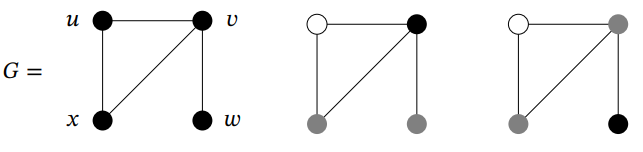
\includegraphics[width=0.8\linewidth]{./fig3/3-2.png}
	\caption{\label{chapter} 一个图与两种着色}
\end{figure}

色数是图论中一个重要的不变量. 但是由它的定义, 它更多地属于极值组合学(研究最小化或最大化约束的结构), 而不是枚举方面. 虽然在这关于$\chi(G)$我们没什么可多说的, 但是我们得说这是最著名的数学定理之一. 称一个图为{\kaishu 平面图}, 如果它可以画在平面上, 没有任何两条边交叉.

\begin{theorem}[四色定理]
	如果$G$ 是平面图, 则$$
	\chi(G) \leq 4.$$
	 $\hfill\square$
\end{theorem}

请注意, 此结果与可以具有任意大色数的普通图形成鲜明对比. 例如, 对完全图有 $\chi\left(K_{n}\right)=n$. 四色定理在 1977 年被 Appel 和 Haken 证明时(在科赫的帮助下)引起了不小的轰动[1,2]. 一方面, 据四色猜想被提出已经过去了100多年. 他们的证明也是第一个大量使用计算机来完成, 所有各种情况的计算和演示不能完全由人工检查.

我们现在转向枚举图着色. 令 $t \in \mathbb{N}$.  $G$ 的色多项式定义为
$$
P(G ; t)=\text { 正常着色数 } c: V \rightarrow[t] \text {. }
$$
这个概念是由 George Birkhoff [13] 提出的. 目前尚不清楚为什么
 $P(G ; t)$ 应该称为多项式, 让我们用图 3.2 中的图形计算它. 按顺序 $u, v, w, x$考虑顶点着色. 顶点$u$的着色有 $t$种选择. 因为$v$不能与$u$染相同的颜色, 于是$v$有$t-1$种选择. 同理,  $w$的选择数为$t-1$. 最后,  $x$的选择方法数为 $t-2$, 因为它不能和$u$ 与 $v$染相同的颜色. 因此, 最终的计数为
\[\quad P(G)=P(G ; t)=t(t-1)(t-1)(t-2)=t^{4}-4 t^{3}+5 t^{2}-2 t.\tag{3.23} \]
这是一个关于 $t$的多项式, 是染色的方法数! 在证明之前, 我们有一些说明. 首先 $P(G ; t)$ 和 $\chi(G)$关系密切, 即当 $0 \leq t<\chi(G)$,  $P(G ; t)=0$ , 但是 $P(G ; \chi(G))>0$. 这是由$P$ 和$\chi$ 的定义得来的, 因为后者是$G$的正常着色存在的最小的非负整数, 前者是对这些着色方法数的计数. 其次, 我们并不总能够用上面方法计算出$P(G ; t)$, 并对整数$k$将其表达为因子 $t-k$的乘积. 例如, 考虑圈 $C_{4}$ , 顶点按顺时针标记为 $u, v, w, x$. 如果我们试着用这种方式计算 $P\left(C_{4} ; t\right)$, 除了顶点  $x$的着色外, 其他都很简单, 因为 $x$与$u$ 和 $w$都相邻. 但是我们不能确定是否 $u$ 和 $w$ 着色相同, 因为它们本身不相邻.

事实证明, 相同的想法可以用于证明$P(G ; t)$ , 并降低计算$P\left(C_{4} ; t\right)$的难度. 考虑图  $G=(V, E)$及一条边$e \in E$. 这个图是由$G$ 删去边$e$得到的, 记作 $G \backslash e$, 它的顶点为 $V$ 且边集为 $E-\{e\}$. 图3.3中中间的图就是例子中删去边  $e=v x$得到的. 在$G$ 中收缩一条边 $e$表示为$G / e$ , 它是通过收缩$e$ 到一个新的顶点 $v_{e}$, 使得 $v_{e}$ 与$e$ 的端点相邻, 其他顶点和边不变. 在我们的示例图中收缩$v x$得到图3.3右侧的图. 下一个引理在 $P(G ; t)$  的研究中至关重要. 理想情况下, 对 $\# E$ 作归纳, 因为$G \backslash e$ 和 $G / e$ 的边都比  $G$的边少.

\begin{figure}[h]
	\centering
	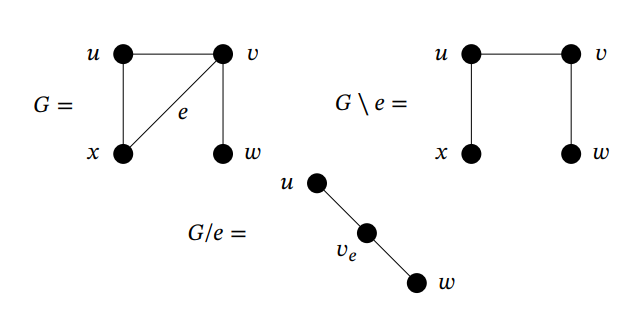
\includegraphics[width=0.8\linewidth]{./fig3/3-3.png}
	\caption{\label{chapter} 删除与收缩}
\end{figure}

\begin{lemma}[删除-收缩引理]
	如果$G$是一个图, $e \in E$, 有
	$$
	P(G ; t)=P(G \backslash e ; t)-P(G / e ; t).
	$$
\end{lemma}

\begin{proof}
我们证明形式$P(G \backslash e)=P(G)+P(G / e)$. 假定	 $e=u v$. 因为$e$ 不出现在$G \backslash e$中, 其正常着色数有两种类型:一种是$c(u) \neq c(v)$ , 另一种是 $c(u)=c(v)$. 如果$c(u) \neq c(v)$,  那么$G \backslash e$的正常着色数等于$G$的正常着色数, 因而有$P(G)$种着色. 当$c(u)=c(v)$时, $G \backslash e$的正常着色与 $G / e$之间也有一个双射, 即对 $v_{e}$着色为和$u$ 与$v$ 相同的颜色, 其他点与$G$着色相同. 这种情况下有$P(G / e)$种着色方式. 利用加法原则, 证毕.
\end{proof}

\begin{theorem}
	对任意图$G$, $P(G ; t)$是关于$t$的多项式.
\end{theorem}

\begin{proof}
	我们对$ |E|$作归纳. 如果$G$没有边, 那么$P(G ; t)=t^{| V|}$, 显然是关于$t$的多项式. 如果 $|E| \geq 1$, 则取边 $e \in E$. 由删除-收缩定理, $P(G ; t)=P(G \backslash e ; t)-P(G / e ; t)$. 由归纳假设,  $P(G \backslash e ; t)$ 与$P(G / e ; t)$ 都是关于$t$的多项式. 因而它们的差也是关于$t$的多项式.
\end{proof}

我们现在可以利用引理3.8.2来计算$C_{4}$的色多项式. 回顾一下符号表示, $P_{n}$ 和 $K_{n}$分别表示$n$个顶点的路和完全图. 现在选出任一边$e \in E\left(C_{4}\right)$, 我们可以运用删除-收缩定理, 然后确定通过逐个顶点着色得到的图的多项式
$$
P\left(C_{4}\right)=P\left(P_{4}\right)-P\left(K_{3}\right)=t(t-1)^{3}-t(t-1)(t-2)=t(t-1)\left(t^{2}-3 t+3\right) .
$$
请注意, 二次因子具有复数根, 因此证实了$P(G)$并不总是有整数的根.

可以使用归纳法和引理 3.8.2 来证明关于$P(G ; t)$的一系列结果. 由于这些证明都是相似的, 我们将它们留给读者. 我们会使用一种非标准的方式写下这个多项式的系数, 这在后面使用比较简单.

\begin{theorem}
	令 $G=(V, E)$, 且
$$
P(G ; t)=a_{0} t^{n}-a_{1} t^{n-1}+a_{2} t^{n-2}-\cdots+(-1)^{n} a_{n} .
$$

(1) $n=|V|$.

(2) mdeg $P(G ; t)=$ $G$的分支数.

(3) 对所有$i$有 $a_{i} \geq 0$ , 且对 $0 \leq i \leq n-$ mdeg $P(G ; t)$有$a_{i}>0$.

(4) $a_{0}=1$且$a_{1}=| E|$.
\end{theorem}
现在我们知道 $P(G ; t)$是一个多项式, 我们想要知道其系数是否存在组合解释, 我们方法的逆可以用来处理序列, 然后找到其生成函数. 对边集 $E$设置一个总序, 如果边$e$在这一序下是小于边$f$的, 记作 $e<f$, 其他符号类似. 如果  $C$ 是 $G$中一个圈, 那么相应的破圈$B$就是在 $E(C)$移除总序中最小的边得到的边集. 回到图3.2中的例子, 令 $b=u v, c=u x, d=v w, e=v x$ , 并设置序$b<c<d<e$. 唯一的圈有边 $b, c, e$ , 且相应的破圈 $B=\{c, e\}$ , 就是一条路的边. 也就是说边集$A \subseteq E$不包含破圈或者说是一个$NBC$集合, 如果$A 6 \supseteq B$对任意破圈 $B$. 令
$$
\mathrm{NBC}_{k}=\mathrm{NBC}_{k}(G)=\{A \subseteq E \mid \# A=k \text {且} A \text { 是一个 } \mathrm{NBC} \text { 集合 }\}
$$
且 $\mathrm{nbc}_{k}=\mathrm{nbc}_{k}(G)=\# \mathrm{NBC}_{k}(G) $. 在我们的例图中,
\begin{table}[h]
	\centering
	\begin{tabular}{l|l|l}
		$k$ & $\mathrm{NBC}_{k}(G)$ & $\mathrm{nbc}_{k}(G)$ \\
		\hline \hline 0 & $\{\emptyset\}$ & 1 \\
		1 & $\{\{b\},\{c\},\{d\},\{e\}\}$ & 4 \\
		2 & $\{\{b, c\},\{b, d\},\{b, e\},\{c, d\},\{d, e\}\}$ & 5 \\
		3 & $\{\{b, c, d\},\{b, d, e\}\}$ & 2 \\
		4 & $\emptyset$ & 0
	\end{tabular}
\end{table}
比较上表的最后一列与$P(G ; t)$ 的系数得出我们下面的结果, 这就是Whitney[99]的结果. 令人惊讶的是结论确实
不取决于赋予边的总序. 我们给出的证明是基于Blass 和 Sagan [16] 的结果.
\begin{theorem}
	如果 $\# V=n$, 那么边集$E$的任意序,
	$$
	P(G ; t)=\sum_{k=0}^{n}(-1)^{k} \mathrm{nbc}_{k}(G) t^{n-k} .
	$$
\end{theorem}

\begin{proof}
将每一个 $A \in \mathrm{NBC}_{k}(G)$与生成子森林联系起来. 那么$A$是无圈的因为任何圈都包含一个破圈. 由定理1.10.2得$A$是一个有$n-k$个分支树的森林. 因此$nbc_{k}(G) t^{n-k}$ 是数对$(A, c)$ 的数目, 其中$A \in \operatorname{NBC}_{k}(G)$ 且$c: V \rightarrow[t]$是$A$的每一个分支上的染色常数. 我们称这样的一个染色为$A$-不正常. 通过令 $\operatorname{sgn}(A, c)=(-1)^{\# A}$使这样的数对集合成为符号集. 因此, 如果我们找到一个在这些数对上的符号反转对合$\iota$, 其固定点集是正的符号, 并且和$G$的正常着色之间存在双射, 即可证明这一定理.

定义$\iota$的固定点集为$(A, c)$使得$A=\emptyset$且$c$是正常的. 这些数对显然具有所需的特性. 对于任何其他数对, $c$不是正常的着色, 因此一定有边$e=u v$ 满足$c(u)=c(v)$. 令$e$是总序中最小的这样的边. 现在定义$\iota(A, c)=(A \Delta\{e\}, c):=\left(A^{\prime}, c\right)$. 很明显 $\iota$是符号反转的. 并且它是一个对合, 因为$c$没有改变, 因此最小的单色
边在一个对及其图像中是相同的. 我们只需要检验$\iota$是定义良好的. 如果$A^{\prime}=A-\{e\}$, 那么很明显$A$仍然是一个NBC集合, 并且$c$是$A^{\prime}$-不正常的. 如果$A^{\prime}=A \cup\{e\}$, 由于$e$连接两个相同颜色的顶点, 所以$c$仍然是$A^{\prime}$-不正常的. 但是利用反证法, 假设$A^{\prime}$不是NBC集. 那么$A^{\prime} \supseteq B$, 其中$B$是一个破圈, 且$e \in B$, 因为$A$是NBC的. 因为$c$是$A^{\prime}$-不正常, $B$中所有的边有顶点着色$c(u)$. 但是$e$是有那样性质的最小的边, 因此通过移除这一条边来得到$B$是不存在的. 因此$A^{\prime}$ 是NBC, $\iota$是定义良好的, 证毕.
\end{proof}

关于色多项式的一个令人惊奇的事情是, 它经常出现在先验没有业务的地方, 因为不涉及图形着色. 我们现在给出两个例子来说明这一点. 回想一下第 2.6 节, 图$G$中的一个方向图$O$, 它是和$G$有相同顶点集的有向图, 通过将$G$的每条边$u v$替换为可能的弧之一$\overrightarrow{u v}$或者 $\overrightarrow{v u}$. 图3.4就是图$G$的两个方向图. 称 $O$是无圈的, 如果它不包含任何有向圈, 令 $\mathcal{A}(G)$和 $a(G)$分别表示图$G$的无圈方向图的集合和计数.  图3.4中第一个方向图是无圈的, 而第二个是有圈的. 圈 $u, v, x, u$的方向图的总数目为 $2^{3}$, 那些形成一个圈的数目是2(顺时针和逆时针). 因为  $v w$ 的任何方向都不可能产生圈, 我们有$a(G)=2\left(2^{3}-2\right)=12$. 我们现在做一些非常奇怪的事情, 将$t=-1$代入
色多项式 (3.23) 并得到 $P(G ;-1)=(-1)(-2)(-2)(-3)=12$. 虽然完全不清楚用-1颜色为图形着色意味着什么, 我们刚刚看到的是
下面的著名的斯坦利定理的例子[85].
\begin{figure}[h]
	\centering
	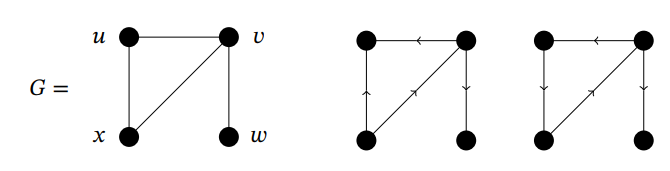
\includegraphics[width=0.8\linewidth]{./fig3/3-4.png}
	\caption{\label{chapter} 一个图的两种方向}
\end{figure}
\begin{theorem}
	对任意图$G$, 顶点数$\# V=n$ , 我们有$$
	P(G ;-1)=(-1)^{n} a(G) \text {. }
	$$
\end{theorem}
\begin{proof}
	我们对$\# E$作归纳, 初始的情况容易验证. 只需验证 $(-1)^{n} P(G ;-1)$ 和$a(G)$满足相同的递推关系. 利用删除-收缩引理, 我们发现只需证明 对固定边$e=u v \in E$有$a(G)=a(G \backslash e)+a(G / e)$. 考虑映射
	$$
	\phi: A(G) \rightarrow A(G \backslash e),
	$$
它将 $O \mapsto O^{\prime}$, 其中 $O^{\prime}$ 通过$O$ 移除 $e$对应的弧得到. 很明显 $O^{\prime}$ 仍然是无圈的, 因此函数是定义良好的.

我们称$\phi$是满射. 假设相反, 存在一些$O^{\prime} \in A(G \backslash e)$使得添加回$\overrightarrow{u v}$得到一个有向圈$C$, 类似地添加回$\overrightarrow{v u}$得到一个有向圈$C^{\prime}$. 那么$(C-\overrightarrow{u v}) \cup\left(C^{\prime}-\overrightarrow{v u}\right)$ 是闭的, 由第一章习题14(2)得到, 有向途径一定包含一条有向圈. 但是第三条有向圈包含在$O^{\prime}$中, 产生矛盾.

如果 $O^{\prime} \in A(G \backslash e)$, 那么由映射的定义, $\# \phi^{-1}\left(O^{\prime}\right) \leq 2$. 从前一段我们知道$\#\phi^{-1}\left(O^{\prime}\right) \geq 1$. 因此 $a(G)=x+2 y$, 其中$x=\#\left\{O^{\prime} \mid \phi^{-1}\left(O^{\prime}\right)=1\right\}$ , $y=\#\left\{O^{\prime} \mid \phi^{-1}\left(O^{\prime}\right)=2\right\} $. 因为 $a(G \backslash e)=x+y$ , 只需证明 $a(G / e)=y$. 我们建立如下双射
$$
\psi:\left\{O^{\prime} \in A(G \backslash e) \mid \phi^{-1}\left(O^{\prime}\right)=2\right\} \rightarrow A(G / e) .
$$

令$Y$为$\psi$的定义域. 如果存在一对边$w u, w v \in E(G)$, 那么任意$O^{\prime} \in Y$ 包含$\overrightarrow{w u}$ 和 $\overrightarrow{w v}$, 或者包含 $\overrightarrow{u w}$和 $\overrightarrow{v w}$. 这是因为在所有其他情形中, 添加回$e$的一个方向将形成$G$的带圈的方向图, 与$\phi^{-1}\left(O^{\prime}\right)=2$矛盾.  因此定义$O^{\prime \prime}=\psi\left(O^{\prime}\right)$为$G / e$的方向图, 它和$O^{\prime}$上不包含新顶点 $v_{e}$的那些弧是一致的, 在形式为$w v_{e}$的那些边和$w u$ 或 $w v$方向相同. (如图所示, 这两个方向要么都朝向 $e$, 要么都远离$e$ ). 证明$\psi$是定义良好的双射留作练习.
\end{proof}

我们应该提到的是, Stanley 实际上证明了对所有负整数$-t$的$P(G ;-t)$进行组合解释的更强结果. 具体细节见练习28(2). 所以, 正如我们在 (1.6) 中看到的二项式系数, 我们有其组合解释的另一个实例. 我们将在下一节更广泛地研究这种现象.

对于色多项式的多变性质的第二个示例, 我们需要假设我们的图$G$有顶点集$[n]$ 以便顶点有一个总序. 令$F$为$G$的生成森林, 并将$F$的每个分支树$T$ 的最小顶点$r$作为根. 称$F$是增的, 如果对于所有的根$r$, 以$r$为起点的路的顶点编号形成增序. 在图3.5中, 是一个图$G$, 其顶点用$[4]$编号, 与两个生成树. 我们称$F_{1}$是增序, 因为任意单元素节点都是增的, 并且对非平凡树, 从根开始的唯一的最大路为$1,2,4$, 显然是一个增序. 另一方面, $F_{2}$非增, 因为有路$1,4,2$.
\begin{figure}[h]
	\centering
	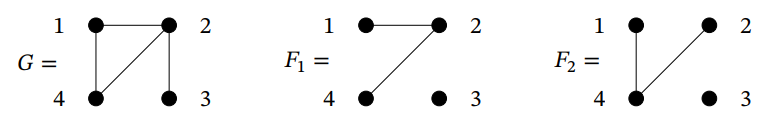
\includegraphics[width=0.8\linewidth]{./fig3/3-5.png}
	\caption{\label{chapter} 一个图与两种生成森林}
\end{figure}

对一个图 $G=(V, E)$ , 我们定义
$$\operatorname{ISF}_{m}(G)=\{F \mid F\text{是} G\text{的有}m\text{条边的生成森林} \},$$且  isf $_{m}(G)=\# \operatorname{ISF}_{m}(G)$. 如果 $\# V=n$, 那么考虑相应的生成多项式
$$
\operatorname{isf}(G)=\operatorname{isf}(G ; t)=\sum_{m=0}^{n}(-1)^{m} \operatorname{isf}_{m}(G) t^{n-m} .
$$
我们用这一公式计算我们的例图. 有零条边或一条边的树都是增的, 因此$\text{isf}_{0}(G)=1$且  $\text{isf}_{1}(G)=\# E=4$. $G$的任意的这样的边对形成一个增森林, 除了图3.5中$F_{2}$那样的边对. 因此 isf$_{2}(G)=\binom{4}{2}-1=5$.  类似地我们可以验证isf$_{3}(G)=2$. 并且 isf$_{4}(G)=0$, 因为$G$本身不是森林. 因此
$$
\operatorname{isf}(G ; t)=t^{4}-4 t^{3}+5 t^{2}-2 t=t(t-1)^{2}(t-2)=P(G ; t) \text {. }
$$
我们并不总是有isf$(G)=P(G)$, 因为前者依赖于顶点的编号(即使我们的符号掩盖了事实), 然而后者并不依赖. 因此, 我们将暂时不考虑它们何时相等, 现在只关注它们在$\mathbb{Z}$上的因式分解, 正如我们将看到的, 它不是巧合. 事实上, 根将是由如下定义的边集的基数
\[
E_{k}=\{i k \in E \mid i<k\},\tag{3.12}
\]
其中 $1 \leq k \leq n$. 在我们的例子中 $E_{1}=\emptyset$ (因为没有顶点比1小), $E_{2}=\{12\}$ $E_{3}=\{23\}$,  $E_{4}=\{14,24\}$.

\begin{lemma}
如果$G$ 有顶点$V=[n]$, 那么一个生成子图$F$是一个增森林当且仅当对于$k \in[n]$它是通过从每个 $E_{k}$中选择最多一条边获得的.
\end{lemma}
\begin{proof}
	对于前一个方向, 利用反证法, 假设$F$包含$i k$ 和 $j k$, 其中$i, j<k$. 因此如果$r$是包含$i, j, k$的树的根, 那么, 由
	增序条件, $i$ 必须是唯一的 $r-k$路径上$k$之前的顶点. 但是$j$也必须如此, 这就产生矛盾.

	对于另一个方向, 我们必须首先验证$F$ 是无圈的. 但是如果$F$包含一个圈$C$, 那么令$k$为其最大顶点. 因此有$i k, j k \in E(C)$, 并且根据最大要求, 有$i, j<k$. 这与假设相矛盾. 类似地, 可以证明如果 $F$ 不是增序, 则可以从相同的 $E_{k}$产生两个边, 证毕.
\end{proof}
 现在证明 Hallam 和 Sagan [41] 的以下结果就很简单了. 这里给出的证明是由 Hallam、Martin 和 Sagan [40] 得到的.
\begin{theorem}
	如果 $G$ 有顶点 $V=[n]$, 那么$$
	\operatorname{isf}(G ; t)=\prod_{k=1}^{n}\left(t-\left|E_{k}\right|\right)
	$$
\end{theorem}
\begin{proof}
	乘积中 $t^{n-m}$的系数是形式$\left|E_{i_{1}}\right|\left|E_{i_{2}}\right| \cdots\left|E_{i_{m}}\right|$ 的所有项的和, 其中$i_{j}$是不同的指标. 但是这个乘积是从每个集合$E_{i_{1}}, E_{i_{2}}, \ldots, E_{i_{m}}$中选出一条边的方法数. 所以, 根据前面引理, 总和是具有$m$条边的增森林的数量, 证毕.
\end{proof}
回到色多项式与增生成森林多项式何时相等的问题, 我们需要下面的定义. 如果 $V$ 的总序$v_{1}, v_{2}, \ldots, v_{n}$使得对所有的$k$, 在总序中在为$v_{k}$之前并与$v_{k}$相邻的顶点集合形成一个团($G$ 的完整子图),  则图 $G$ 具有完美消除序 (peo). 乍一看, 这个定义似乎很奇怪, 但是它在各种图理论环境中很有用. 回到我们的例子, 我们看到序$1,2,3,4$是一个完美消除序 , 因为 1 与之前的顶点不相邻, 顶点 2 和 3 都与单个先前的顶点相邻, 即 $K_{1}$, 并且 4 与 1 和 2 相邻, 这形成一条边, 也即$K_{2}$. 我们可以证明来自 [40]的另一个结果.
 \begin{lemma}
 	令$G$ 顶点$V=[n]$. 将$G$的边写作$i j$其中 $i<j$, 并将它们按字典序排列. 对所有的$m \geq 0$, 我们有$$
 	\operatorname{ISF}_{m}(G) \subseteq \operatorname{NBC}_{m}(G) .
 	$$此外, 对所有的$m$上面两个集合相等当且仅当$[n]$ 上的自然顺序是完美消除序.
 \end{lemma}

\begin{proof}
	为了证明包含关系, 我们假设$F$ 是一个增的生成森林, 它包含破圈$B$, 并导出矛盾. 按边的字典序, $B$必须是形式为 $v_{1}, v_{2}, \ldots, v_{l}$的路, 其$v_{1}=\min \left\{v_{1}, \ldots, v_{l}\right\}$, 且$v_{2}>v_{l}$. 所以一定存在一个最小指标 $i \geq 2$使得$v_{i}>v_{i+1}$. 随之有 $v_{i-1}, v_{i+1}<v_{i}$, 所以 $B$的两条相应的边与引理 3.8.7 矛盾.

	对于第二个陈述的前一个方向, 我们必须证明如果$i, j<k$并且$i k, j k \in E(G)$, 那么$i j \in E(G)$. 再利用引理3.8.7, $\{i k, j k\}$不是增生成森林的边集. 因此, 通过假定的相等性, 这个集合必须包含一个破圈. 由于只有两条边, 这一边集一定是破圈, 并且$i j \in E(G)$一定是用来形成圈的边. 另一方向的证明留作练习.
\end{proof}
从这个结果, 我们立即得出以下结论.
\begin{theorem}
	令$G$ 顶点$V=[n]$. 那么$\operatorname{isf}(G ; t)=P(G ; t)$当且仅当$[n]$上的自然序是一个完美消除序. $\hfill\square$
\end{theorem}
\section{组合互反性}

将一个负参数代入一个计数函数得到一个符号乘另一个计数函数, 那么这就称为组合互反. 这一概念是由Stanley[86]引入和研究的. 我们已经在等式(1.6)与定理3.8.6中看到了两个例子(更一般地, 见本章练习28). 在这里, 我们将递归与有理生成函数联系起来. 请参阅 Beck 和 Sanyal [5] 的关于该问题的论述.

在陈述一个一般定理之前, 我们回到第 3.6 节开始的例子. 也即如下定义的序列$a_{0}=2$, 且当$n \geq 1$时$a_{n}=3 a_{n-1}$. 我们可以将这一递推关系的定义域扩展到所有的整数$n$, 在这种情况下可以得到 $2=a_{0}=3 a_{-1}$, 因此$a_{-1}=2 / 3$. 那么$2 / 3=a_{-1}=3 a_{-2}$, 于是得到$a_{-2}=2 / 3^{2}$, 以此类推. 作简要的归纳得到当$n \leq 0$ 有 $a_{n}=2 \cdot 3^{n}$, 与$n \geq 0$时一样. 我们也可对这一序列的负指标部分计算生成函数, 从$a_{-1}$开始计算, 得到几何级数
$$
\sum_{n \geq 1} a_{-n} x^{n}=\sum_{n \geq 1} \frac{2 x^{n}}{3^{n}}=\frac{2 x / 3}{1-x / 3}=\frac{2 x}{3-x} .
$$
将其与(3.12)中的式子 $f(x)=\sum_{n \geq 0} a_{n} x^{n}$比较得到
$$
-f(1 / x)=\frac{-2}{1-3 / x}=\frac{2 x}{3-x}=\sum_{n \geq 1} a_{-n} x^{n} .
$$

读者应该对写 $f(1 / x)$有些疑虑, 因为我们已经指出$x$在$\mathbb{C}[[x]]$中没有逆. 事实上, 如果我们使用定义$f(x)=\sum_{n \geq 0} a_{n} x^{n}$, 那么$f(1 / x)=\sum_{n \geq 0} a_{n} / x^{n}$, 这不是一个形式幂级数. 但是如果$f(x)$可以被表达成有理函数的形式, 即$f(x)=p(x) / q(x)$, 其中$\operatorname{deg} p(x) \leq$ $\operatorname{deg} q(x):=d$, 那么作如下替换就有意义. 因为$q(x)$度为 $d$, 我们知道$x^{d} q(1 / x)$也是一个多项式, 并且是可逆的, 因为它的常数项不为零(定理 3.3.1). 此外, $x^{d} p(1 / x)$ 也是一个多项式, 因为 $d \geq \operatorname{deg} p(x)$. 所以我们可以定义
\[
f(1 / x)=\frac{x^{d} p(1 / x)}{x^{d} q(1 / x)},\tag{3.25}
\]
它仍在形式幂级数环中. 在这样定义下, 下面的结果就有意义.

\begin{theorem}
	假设$a_{n}$是一个序列,  $n \in \mathbb{Z}$满足(3.18)中常系数的线性递推关系. 令$f(x)=\sum_{n \geq 0} a_{n} x^{n}$, 我们有$$
	\sum_{n \geq 1} a_{-n} x^{n}=-f(1 / x)
	$$
\end{theorem}
\begin{proof}
	由(3.25), 要证明该定理只需证明$$
	x^{d} q(1 / x) \sum_{n \geq 1} a_{-n} x^{n}=-x^{d} p(1 / x).
	$$注意由(3.20)式, 我们有$$
	x^{d} q(1 / x)=x^{d}+c_{1} x^{d-1}+c_{2} x^{d-2}+\cdots+c_{d} .
	$$因此, 如果$m \geq 1$, 那么利用(3.18)及$x^{d} p(1 / x)$的度至多为$d$, 得$$
	\begin{aligned}
	{\left[x^{m+d}\right] x^{d} q(1 / x) \sum_{n \geq 1} a_{-n} x^{n} } &=a_{-m}+c_{1} a_{-m-1}+c_{2} a_{-m-2}+\cdots+c_{d} a_{-m-d} \\
	&=0 \\
	&=\left[x^{m+d}\right]\left(-x^{d} p(1 / x)\right) .
	\end{aligned}
	$$
	类似地, 我们可以证明该不等式对$-d \leq m \leq0$ 仍成立. 证毕.
\end{proof}
为了说明这一定理, 我们考虑负的二项式展开. 如果固定$n \geq 1$, 应用定理3.4.2及等式(3.16), 得
$$
f(x):=\frac{1}{(1-x)^{n}}=\sum_{k \geq 0}\left(\left(\begin{array}{l}
n \\
k
\end{array}\right)\right) x^{k}=\sum_{k \geq 0}\left(\begin{array}{c}
n+k-1 \\
n-1
\end{array}\right) x^{k}.
$$
注意因为$n$是固定的, 我们将$\binom{n+k-1}{n-1}$看作关于 $k$的函数. 在二项式系数中将 $k$替换为 $-k$, 我们考虑相应的生成函数
$$
g(x)=\sum_{k \geq 1}\binom{n-k-1}{n-1}x^{k}.
$$
注意到当$1 \leq k<n$时 $\binom{n-k-1}{n-1}=0$, 因为$0 \leq n-k-1<n-1$. 所以 $x^{n}$可以从 $g(x)$分解出来, 使用(1.6)和上面的负
二项式展开, 得到
$$
\begin{aligned}
g(x) &=x^{n} \sum_{k \geq n}\left(\begin{array}{c}
n-k-1 \\
n-1
\end{array}\right) x^{k-n} \\
&=x^{n} \sum_{j \geq 0}\left(\begin{array}{c}
-j-1 \\
n-1
\end{array}\right) x^{j} \\
&=(-1)^{n-1} x^{n} \sum_{j \geq 0}\left(\left(\begin{array}{c}
j+1 \\
n-1
\end{array}\right)\right) x^{j} \\
&=(-1)^{n-1} x^{n} \sum_{j \geq 0}\left(\begin{array}{c}
n+j-1 \\
n-1
\end{array}\right) x^{j} \\
&=\frac{(-1)^{n-1} x^{n}}{(1-x)^{n}} .
\end{aligned}
$$
另一方面, 我们可以应用定理3.9.1将$g(x)$写作
$$
g(x)=\frac{-1}{(1-1 / x)^{n}}=\frac{-x^{n}}{(x-1)^{n}}=\frac{(-1)^{n-1} x^{n}}{(1-x)^{n}},
$$
得到同样的结果, 但是计算更少.

\section{习题}
1.用三种方式证明对 $n \in \mathbb{N}$
$$
\sum_{k=0}^{n} 2^{k}\binom{n}{k}=3^{n}.
$$
(1)应用二项式定理。
(2)应用组合解释。
(3)对任意$c \in \mathbb{N}$,通过把$2^{k}$替换为$c^{k}$将等式一般化,用二项式定理及组合解释给出证明。

2.对$m, n, k \in \mathbb{N}$,证明
$$
\left(\begin{array}{c}
m+n \\
k
\end{array}\right)=\sum_{l \geq 0}\left(\begin{array}{c}
m \\
l
\end{array}\right)\left(\begin{array}{c}
n \\
k-l
\end{array}\right)
$$
in three ways: by induction, using the Binomial Theorem, and using a combinatorial argument.
(3) Let $x_{1}, \ldots, x_{m}$ be variables. Prove the multinomial coefficient identity
$$
\sum_{n_{1}+\cdots+n_{m}=n}\left(\begin{array}{c}
n \\
n_{1}, \ldots, n_{m}
\end{array}\right) x_{1}^{n_{1}} \cdots x_{m}^{n_{m}}=\left(x_{1}+\cdots+x_{m}\right)^{n}
$$
in three ways:
(a) by inducting on $n$,
(b) by using the Binomial Theorem and inducting on $m$,
(c) by a combinatorial argument.
(4) (a) Prove Theorem 3.1.2.
(b) Use this generating function to rederive Corollary 1.5.3.
(5) (a) Recall that an inversion of $\pi \in P([n])$ is a pair $(i, j)$ with $i<j$ and $\pi_{i}>\pi_{j}$ and we call $\pi_{i}$ the maximum of the inversion. The inversion table of $\pi$ is $I(\pi)=$ $\left(a_{1}, a_{2}, \ldots, a_{n}\right)$ where $a_{k}$ is the number of inversions with maximum $k$. Show that $0 \leq a_{k}<k$ for all $k$ and that
$$
\operatorname{inv} \pi=\sum_{k=1}^{n} a_{k}
$$
(b) Let
$$
\mathcal{I}_{n}=\left\{\left(a_{1}, a_{2}, \ldots, a_{n}\right) \mid 0 \leq a_{k}<k \text { for all } k\right\} .
$$
Show that the map $\pi \mapsto I(\pi)$ is a bijection $P([n]) \rightarrow \mathcal{I}_{n}$.
(c) Use part (b) and weight-generating functions to rederive Theorem $3.2 .1$.
(6) Let st: $\Im_{n} \rightarrow \mathbb{N}$ be a statistic on permutations. Recall that for a permutation $\pi$ we let $\operatorname{Av}_{n}(\pi)$ denote the set of permutations in $\Im_{n}$ avoiding $\pi$. Say that permutations $\pi, \sigma$ are st-Wilf equivalent, written $\pi \stackrel{\text { st }}{\equiv} \sigma$, if for all $n \geq 0$ we have equality of the

generating functions
$$
\sum_{\tau \in \mathrm{Av}_{n}(\pi)} q^{\mathrm{st} \tau}=\sum_{\tau \in \mathrm{Av}_{n}(\sigma)} q^{\mathrm{st} \tau}
$$
(a) Show that if $\pi$ and $\sigma$ are st-Wilf equivalent, then they are Wilf equivalent.
(b) Show that
$$
132 \stackrel{\text { inv }}{\equiv 13}
$$
and
$$
231 \stackrel{\text { inv }}{\equiv} 312
$$
and that there are no other inv-Wilf equivalences between two permutations in $\mathfrak{~}_{3}$.
(c) Show that
$$
\begin{aligned}
&132 \stackrel{\text { maj }}{\equiv} 231 \\
&213 \stackrel{\text { maj }}{\equiv} 312
\end{aligned}
$$
and
and that there are no other maj-Wilf equivalences between two permutations in $\subseteq_{3}$.
(7) (a) Prove that
$$
\left[\begin{array}{l}
n \\
k
\end{array}\right]=\left[\begin{array}{c}
n \\
n-k
\end{array}\right]
$$
in three ways: using the $q$-factorial definition, using the interpretation in terms of integer partitions, and using the interpretation in terms of subspaces.
(b) Prove the second recursion in Theorem 3.2.3 in two ways: by mimicking the proof of the first recursion and by using the first recursion in combination with part (a).
(c) If $S \subseteq[n]$, then let $\Sigma S$ be the sum of the elements of $S$. Give two proofs of the following $q$-analogue of the fact that $\#\left(\begin{array}{c}{[n]} \\ k\end{array}\right)=\left(\begin{array}{c}n \\ k\end{array}\right)$ :
$$
\sum_{S \in\left(\begin{array}{c}
	(n) \\
	k
	\end{array}\right)} q^{\Sigma S}=q^{\left(\begin{array}{c}
	k+1 \\
	2
	\end{array}\right)}\left[\begin{array}{l}
n \\
k
\end{array}\right]_{q},
$$
one proof by induction and the other using Theorem 3.2.5.
(d) Give two other proofs of Theorem 3.2.6: one by inducting on $n$ and one by using Theorem 3.2.5.
(8) (a) Reprove Theorem $3.2 .4$ in two way: using integer partitions and using subspaces.
(b) The Negative $q$-Binomial Theorem states that
$$
\frac{1}{(1-t)(1-q t)\left(1-q^{2} t\right) \ldots\left(1-q^{n-1} t\right)}=\sum_{k \geq 0}\left[\begin{array}{c}
n+k-1 \\
k
\end{array}\right] t^{k}
$$
Give three proofs of this result: inductive, using integer partitions, and using subspaces.

(9) (a) Given $n_{1}+n_{2}+\cdots+n_{m}=n$, define the corresponding $q$-multinomial coefficient to be
$$
\left[n_{1}, n_{2}, \ldots, n_{m}\right]_{q}=\frac{[n]_{q}}{\left[n_{1}\right]_{q} !\left[n_{2}\right]_{q} ! \ldots\left[n_{m}\right]_{q} !}
$$
if all $n_{i} \geq 0$ or zero otherwise. Prove that
$$
\begin{aligned}
&{\left[n_{1}, n_{2}, \ldots, n_{m}\right]_{q}} \\
&=\sum_{i=1}^{m} q^{n_{1}+n_{2}+\cdots+n_{i-1}}\left[\begin{array}{c}
n-1 \\
n_{1}, \ldots, n_{i-1}, n_{i}-1, n_{i+1}, \ldots, n_{m}
\end{array}\right]_{q}
\end{aligned}
$$
(b) Define inversions, descents, and the major index for permutations (linear orderings) of the multiset $M=\left\{\left\{1^{n_{1}}, 2^{n_{2}}, \ldots, m^{n_{m}}\right\}\right\}$ exactly the way as was done for permutations without repetition. Let $P(M)$ be the set of permutations of M. Prove that
$$
\sum_{\pi \in P(M)} q^{\mathrm{inv} \pi}=\sum_{\pi \in P(M)} q^{\mathrm{maj} \pi}=\left[\begin{array}{c}
n \\
\left.n_{1}, n_{2}, \ldots, n_{m}\right]_{q}
\end{array}\right.
$$
(c) Let $V$ be a vector space over $\mathbb{F}_{q}$ of dimension $n$. Assume $S=\left\{s_{1}<\cdots<s_{m}\right\} \subseteq$ $\{0,1, \ldots, n\}$. Then a flag of type $S$ is a chain of subspaces
$$
F: W_{1}<W_{2}<\cdots<W_{m} \leq V
$$
such that $\operatorname{dim} W_{i}=s_{i}$ for all $i$. The reason for this terminology is that when $n=2$ and $S=\{0,1,2\}$, then $F$ consists of a point (the origin) contained in a line contained in a plane which could be viewed as a drawing of a physical flag with the point being the hole in the ground, the line being the flag pole, and the plane being the cloth flag itself. Give two proofs that
$$
\#\{F \text { of type } S\}=\left[s_{1}, s_{2}-s_{1}, s_{3}-s_{2}, \ldots, s_{m}-s_{m-1}, n-s_{m}\right]_{q} \text {, }
$$
one by mimicking the proof of Theorem $3.2 .6$ and one by induction on $m$.
(10) (a) Prove that in $C[[x]]$ we have $e^{k x}=\left(e^{x}\right)^{k}$ for any $k \in \mathbb{N}$.
(b) Define formal power series for the trigonometric functions using their usual Taylor expansions. Prove that in $C[[x]]$ we have $\sin ^{2} x+\cos ^{2} x=1$ and $\sin 2 x=2 \sin x \cos x$.
(c) If one is given a sequence $a_{0}, a_{1}, a_{2}, \ldots$ and defines
$$
f_{k}(x)=a_{k} x^{k},
$$
then show that $\sum_{k \geq 0} f_{k}(x)=f(x)$ where $f(x)=\sum_{k \geq 0} a_{k} x^{k}$.
(d) Prove the backwards direction of Theorem $3.3 .2$.
(e) Use Theorems $3.3 .1$ and $3.3 .3$ to reprove that $1 / x$ and $e^{1+x}$ are not well-defined in $\mathbb{C}[[x]]$.
(f) Prove Theorem 3.3.4
(11) Prove that if $S, T$ are summable sets, then so is $S \times T$.

(12) Say that $f(x) \in \mathbb{C}[[x]]$ has a square root if there is $g(x) \in \mathbb{C}[[x]]$ such that $f(x)=$ $g(x)^{2}$
(a) Prove that $f(x)$ has a square root if and only if mdeg $f(x)$ is even.
(b) Show that as formal power series
$$
(1+x)^{1 / 2}=\sum_{k \geq 0}\left(\begin{array}{c}
1 / 2 \\
k
\end{array}\right) x^{k}
$$
(c) Show that as formal power series
$$
\left(e^{x}\right)^{1 / 2}=\sum_{k \geq 0} \frac{x^{k}}{2^{k} k !}
$$
(d) Generalize the previous parts of this exercise to $m$ th roots for $m \in \mathbb{P}$.
(13) Give a second proof of Theorem $3.4 .2$ by using induction.
(14) Prove Theorem $3.4 .3$.
(15) Prove Theorem 3.5.1.
(16) (a) Finish the proof of Theorem $3.5 .3$ (a).
(b) Give a second proof of Theorem $3.5 .3$ (b) by using Theorem $3.2 .5$.
(c) Show that the generating function for the number of partitions of $n$ with largest part $k$ equals the generating function for the number of partitions of $n$ with exactly $k$ parts and that both are equal to the product
$$
\frac{x^{k}}{(1-x)\left(1-x^{2}\right) \cdots\left(1-x^{k}\right)}
$$
(d) The Durfee square of a Young diagram $\lambda$ is the largest square partition $\left(d^{d}\right)$ such that $\left(d^{d}\right) \subseteq \lambda$. Use this concept to prove that
$$
\sum_{n \geq 0} p(n) x^{n}=\sum_{d \geq 0} \frac{x^{d^{2}}}{(1-x)^{2}\left(1-x^{2}\right)^{2} \cdots\left(1-x^{d}\right)^{2}}
$$
(17) Let $a_{n}$ be the number of integer partitions of $n$ such that any part $i$ is repeated fewer than $i$ times and let $b_{n}$ be the number of integer partitions of $n$ such that no part is a square. Use generating functions to show that $a_{n}=b_{n}$ for all $n$.
(18) Given $m \geq 2$, use generating functions to show that the number of partitions of $n$ where each part is repeated fewer than $m$ times equals the number of partitions of $n$ into parts not divisible by $m$. Note that bijective proofs of this result were given in Exercise 15 of Chapter 2 .
(19) (a) Show that $F_{n}$ is the closest integer to
$$
\frac{1}{\sqrt{5}}\left(\frac{1+\sqrt{5}}{2}\right)^{n}
$$
for $n \geq 1$.
(b) Prove that
$$
F_{n}^{2}= \begin{cases}F_{n-1} F_{n+1}+1 & \text { if } n \text { is odd, } \\ F_{n-1} F_{n+1}-1 & \text { if } n \text { is even }\end{cases}
$$
in two ways: using equation ( $(3.14)$ and by a combinatorial argument.

(20) (a) Use the algorithm in Section $2.6$ to rederive Theorem 3.1.1.
(b) Complete the proof of Theorem 3.6.1.
(c) Give a second proof of Theorem 3.6.1 using Theorem $3.1 .2$
(d) Prove Theorem 3.6.2.
(e) Let $s$ be the infinite matrix with rows and columns indexed by $\mathbb{N}$ and with $s(n, k)$ being the entry in row $n$ and column $k$. Similarly define $S$ with entries $S(n, k)$. Show that $S s=s S=I$ where $I$ is the $\mathbb{N} \times \mathbb{N}$ identity matrix. Hint: Use Theorems 3.6.1 and 3.6.2.
(21) Given $n \in \mathbb{N}$ and $k \in \mathbb{Z}$, define the corresponding q-Stirling number of the second kind by $S[0, k]=\delta_{0, k}$ and, for $n \geq 1$,
$$
S[n, k]=S[n-1, k-1]+[k]_{q} S[n-1, k] .
$$
(a) Show that
$$
\sum_{n \geq 0} S[n, k] x^{n}=\frac{x^{k}}{\left(1-[1]_{q} x\right)\left(1-[2]_{q} x\right) \cdots\left(1-[k]_{q} x\right)} .
$$
(b) All set partitions $\rho=B_{1} / B_{2} / \ldots / B_{k}$ in the rest of this problem will be written in standard form, which means that
$$
1=\min B_{1}<\min B_{2}<\cdots<\min B_{k} .
$$
An inversion of $\rho$ is a pair $\left(b, B_{j}\right)$ where $b \in B_{i}$ for some $i<j$ and $b>\min B_{j}$. We let inv $\rho$ be the number of inversions of $\rho$. For example, $\rho=B_{1} / B_{2} / B_{3}=$ $136 / 25 / 4$ has inversions $\left(3, B_{2}\right),\left(6, B_{2}\right),\left(6, B_{3}\right)$, and $\left(5, B_{3}\right)$ so that inv $\rho=4$. Show that
$$
S[n, k]=\sum_{\rho \in S([n], k)} q^{\operatorname{inv} \rho .}
$$
(c) A descent of a set partition $\rho$ is a pair $\left(b, B_{i+1}\right)$ where $b \in B_{i}$ and $b>\min B_{j}$. We let des $\rho$ be the number of descents of $\rho$. In the previous example, $\rho$ has descents $\left(3, B_{2}\right),\left(6, B_{2}\right)$, and $\left(5, B_{3}\right)$ so that des $\rho=3$. The descent multiset of $\rho$ is denoted Des $\rho$ and is the multiset
$$
\left\{\left\{1^{d_{1}}, 2^{d_{2}}, \ldots, k^{d_{k}} \mid \text { for all } i, d_{i}=\text { number of descents }\left(b, B_{i+1}\right)\right\}\right\} \text {. }
$$
The major index of $\rho$ is
$$
\text { maj } \rho=\sum_{i \in \operatorname{Des} \rho} i=d_{1}+2 d_{2}+\cdots+k d_{k} \text {. }
$$
In our running example Des $\rho=\left\{\left\{1^{2}, 2^{1}\right\}\right\}$ so that maj $\rho=1+1+2=4$. Show that
$$
S[n, k]=\sum_{\rho \in S([n], k)} q^{\text {maj } \rho .}
$$
(22) Given $n \in \mathbb{N}$ and $k \in \mathbb{Z}$, define the corresponding signless $q$-Stirling number of the first kind by $c[0, k]=\delta_{0, k}$ and, for $n \geq 1$,
$$
c[n, k]=c[n-1, k-1]+[n-1]_{q} c[n-1, k]
$$
(a) Show that
$$
\sum_{k \geq 0} c[n, k] x^{k}=x\left(x+[1]_{q}\right)\left(x+[2]_{q}\right) \cdots\left(x+[n-1]_{q}\right) .
$$

(b) The standard form of $\pi \in \mathfrak{S}_{n}$ is $\pi=\kappa_{1} \kappa_{2} \cdots \kappa_{k}$ where the $\kappa_{i}$ are the cycles of $\pi$,
$$
\min \kappa_{1}<\min \kappa_{2}<\cdots<\min \kappa_{k} \text {, }
$$
and each $\kappa_{i}$ is written beginning with $\min \kappa_{i}$. Define the cycle major index of $\pi$ to be maj ${ }_{c} \pi=$ maj $\pi^{\prime}$ where $\pi^{\prime}$ is the permutation in one-line form obtained by removing the cycle parentheses in the standard form of $\pi$. If, for example, $\pi=(1,7,2)(3,6,8)(4,5)$, then $\pi^{\prime}=17236845$ so that maj $_{c} \pi=2+6=8$. Show that
$$
c[n, k]=\sum_{\pi \in c([n], k)} q^{\mathrm{maj}_{\mathrm{c}} \pi} .
$$
(23) Reprove the formula
$$
C(n)=\frac{1}{n+1}\left(\begin{array}{c}
2 n \\
n
\end{array}\right)
$$
by using Theorem $2.6 .3$.
(24) (a) Show that if $k, l \in \mathbb{N}$ are constants, then $\left(\begin{array}{c}n+l \\ k\end{array}\right)$ is a polynomial in $n$ of degree $k$.
(b) Show that the polynomials
$$
\left(\begin{array}{l}
n \\
0
\end{array}\right),\left(\begin{array}{c}
n+1 \\
1
\end{array}\right),\left(\begin{array}{c}
n+2 \\
2
\end{array}\right), \ldots
$$
form a basis for the algebra of polynomials in $n$.
(c) Use part (a) to complete the proof of Theorem 3.7.1.
(25) Redo the solution for the first recursion in Section $3.6$ as well as the one for $F_{n}$ using the method of undetermined coefficients.
(26) Prove for the $n$-cycle that
$$
P\left(C_{n} ; t\right)=(t-1)^{n}+(-1)^{n}(t-1)
$$
in two ways: using deletion-contraction and using NBC sets.
(27) Prove Theorem 3.8.4 using induction and give a second proof of parts (b)-(d) using NBC sets.
(28) (a) Complete the proof of Theorem
(b) Let $G=(V, E)$ be a graph and $t \in \mathbb{P}$. Call an acyclic orientation $O$ and a (not necessarily proper) coloring $c: V \rightarrow[t]$ compatible if, for all arcs $\overrightarrow{u v}$ of $O$, we have $c(u) \leq c(v)$. Show that if $\# V=n$, then
$$
P(G ;-t)=(-1)^{n}(\text { number of compatible pairs }(O, c)) \text {. }
$$
(c) Show that Theorem $3.8 .6$ is a special case of part (b).
(29) Finish the proofs of Lemma $3.8 .7$ and Lemma 3.8.9.
(30) (a) Call a permutation $\sigma$ which avoids $\Pi=\{231,312,321\}$ tight. Show that $\sigma$ is tight if and only if $\sigma$ is an involution having only 2 -cycles of the form $(i, i+1)$ for some $i$.
(b) Let $G$ be a graph with $V=[n]$. Call a spanning forest $F$ of $G$ tight if the sequence of labels on any path starting at a root of $F$ avoids $\Pi$ as in part (a). Let
$\operatorname{TSF}_{m}(G)=\{F \mid F$ is a tight spanning forest of $G$ with $m$ edges $\} .$

Show that if $G$ has no 3 -cycles, then for all $m \geq 0$
$$
\operatorname{TSF}_{m}(G) \subseteq \mathrm{NBC}_{m}(G) .
$$
(c) A candidate path in a graph $G$ with no 3 -cycles is a path of the form
$$
a, c, b, v_{1}, v_{2}, \ldots, v_{m}=d
$$
such that $a<b<c, m \geq 1$, and $v_{m}$ is the only $v_{i}$ smaller than $c$. A total order on $V(G)$ is called a quasiperfect ordering (qpo) if every candidate path satisfies the following condition: either $a d \in E(G)$, or $d<b$ and $c d \in E(G)$. Consider the generating function
$$
\operatorname{tsf}(G ; t)=\sum_{m \geq 0}(-1)^{m} \operatorname{tsf}_{m}(G) t^{n-m} .
$$
Show that $\operatorname{tsf}(G ; t)=P(G ; t)$ if and only if the natural order on $[n]$ is a qpo.
(31) Fill in the details of the case $-d \leq m \leq 0$ in the proof of Theorem 3.9.1.
(32) (a) Extend the Fibonacci numbers $F_{n}$ to all $n \in \mathbb{Z}$ by insisting that their recursion continue to hold for $n<0$. Show that if $n \geq 0$, then
$$
F_{-n}=(-1)^{n-1} F_{n} .
$$
(b) Find $\sum_{n \geq 1} F_{-n} x^{n}$ in two ways: by using part (a) and by using Theorem $3.9 .1$.




\end{document}